\chapter{Méthodes et outils}
\label{chap:Méthodes et outils}
Outre ce qui est présenté spécifiquement pour la pensée en cycle de vie, nous allons détailler ci-après les méthodes et outils employés ou analysés dans nos travaux.
Nous observerons donc~:\\
- les outils actuels de l'\gls{ACV} avec les bases de données, les outils de modélisation \ref{sec:Outils de modélisation en ACV}, complétant l'état de l'art et soulignant des caractéristique pour la reconception (\ref{chap:ACV, la (re)conception d'un outil})~;\\
%les outils du web sémantique \ref{} ;
%, de nettoyage et traitement de donnée\ref{} ;
- les outils et la théorie de la \emph{conception}, plus particulièrement la conception fonctionnelle \ref{sec:Méthodologies et théorie de la conception}, employés dans la reconception (\ref{chap:ACV, la (re)conception d'un outil}) mais aussi dans la détermination des unités fonctionnelles et l'observation générale des systèmes industriels, \emph{donc des outils de pratique de l'ACV}~;\\
- l'\acrlong{ADMC} (\ref{sec:ADMC}) pour son inclusion dans l'\gls{ACV} re-conçue.

\section{Outils de modélisation en ACV}
\label{sec:Outils de modélisation en ACV}
Pour produire les différents niveaux d'information comme vu dans la figure~\ref{fig:ILCD_principe_3_niveaux_information.png}, la communauté de la discipline a produit des logiciels.

\begin{itemize}
\item Voyons d'abord les programmes de modélisation, avec ou sans interface graphique, c'est à dire les outils pour~:
\begin{itemize}[noitemsep]
\item la construction du modèle de chaîne de valeur,
\item la caractérisation des impacts,
\item et l'interprétation.
\end{itemize} 
\item Puis nous observerons les bases de données.
Il s'agit de recueils des émissions et consommations de procédés.
Nous pouvons pour compléter le langage de la discipline dire que les \emph{flux élémentaires et de produits} sont regroupés dans des \emph{\textbf{bases d'inventaires} dits '\textbf{secondaires}'.}
Ceux-ci supportent l'allègement de la charge d'\textbf{inventaire primaire} à réaliser lors de chaque cas d'étude.
Mais les bases d'inventaires incluent également des modèles de mécanismes environnementaux et leurs facteurs d'impacts.
Les modélisations des mécanismes environnementaux sont reprises de façon linéaire (facteurs d'impacts constants) au sein de méthodes d'impacts, associées ou indépendantes de bases secondaires.
\end{itemize} 
Nous nous pencherons tout d'abord sur l'aspect informatique puis informationnel en nous concentrant sur les méthodes d'impacts.
\subsection{L'informatique de l'ACV}
\label{subsec:L'informatique de l'ACV}
\subsubsection{L'interface de modélisation}
\label{subsec:L'interface de modélisation}
La modélisation est généralement conduite via une interface graphique recevant les deux premiers éléments listés en introduction (inventaires secondaires et méthodes d'impacts) et fournissant des outils pré-définis pour le calcul et l'interprétation des caractérisations.

Dans la vaste \href{http://eplca.jrc.ec.europa.eu/ResourceDirectory/faces/tools/toolList.xhtml}{liste des logiciels de la commission européenne} (61 éléments), si des classiques comme Simapro, GaBi ou Umberto ont voix au chapitre, des alternatives en codes ouverts tel \href{http://brightwaylca.org/}{BrightWayLCA}~\cite{mutel_brightway2_2012} et \href{http://www.openlca.org/}{OpenLCA}~\cite{ciroth_ict_2007} n'y figurent pas\footnote{Absence constaté lors de la consultation de ces pages et cela malgré l’existence de bientôt 10 ans d'OpenLCA.}.

De façon générale, les interfaces graphiques présentent, un bandeau de navigation dans les bases secondaires et méthodes d'impact, une arborescence pour la construction du projet de modélisation (unités, flux, procédés, systèmes, projets, scénarios, caractérisation \ldots), une fenêtre d'observation ou/et modélisation du système à l'étude (schéma bloc des procédés et flux).
Développées semble-t-il principalement pour l'activité de consulting, ces interfaces (logiciels) s'accompagnent souvent de programmes intégrés d'édition de rapports d'études.

\href{http://brightwaylca.org/}{BrightWayLCA} est un outil python en ligne de commande et \href{http://www.openlca.org/}{OpenLCA} permet également une interaction par scripte et console.
Des versions 'développeurs' sont également disponibles pour les codes fermés qui sans doute disposent de telles fonctionnalité, mais le prix de vente n'est évidement plus le même.
Mais de façon plus problématique en recherche (pas en conseil si cela n'intéresse pas le client), c'est la fermeture du code et la non-reproductibilité vérifiable (rédhibitoire pour la production \emph{scientifique}).

L'acquisition d'une licence de ces outils (globalement propriétaire) s'accompagne souvent de celle de la base de données attenante (Simapro - ecoinvent ; GaBi - GaBi).
Le choix sur la modélisation entraîne donc une orientation sur les types de données employées (unitaires, ou agrégées).

Les capacités d'interactions sur ces outils sont probablement le fruit direct des choix de format de données.
Des bases non requêtables (queryable) ou au format non ouvert conditionnent la possibilité et la difficulté de développer ces fonctionnalités.
En tout cas il y a une forte importance suivant les orientations principales actuelles du rôle de l'analyste avec une faible capacité à la reproduction et vérification des travaux.
\subsubsection{Bases de données}
\label{subsubsec:Bases de données}
\citeauthor{sayan_contribution_2011} a réalisé une études des bases de données. % dans \citetitle{sayan_contribution_2011}.
Elle y dénombre 40 bases avec des états et des contenus très variables.
Ses annexes, que nous ne reproduisons pas par commodité et puisqu'elles sont librement accessible (\href{https://uwspace.uwaterloo.ca/handle/10012/6336}{ici})
avec notamment les tableaux sur les bases analysées\footnote{
Table 2-2 Databases Reviewed ;
Table 2-3 Database Survey – Relationship Between Access and Facilitator Type ;
APPENDIX A. LCA DATABASE REVIEW COLLECTED DATA ;
Table A-1 The Databases Reviewed ;
Table A-2 Access
},
nous éclairent de façon synthétique sur ce paysage informatique.

\paragraph{L'accès et les droits d'usage} font partie des éléments audité par \citeauthor{sayan_contribution_2011}.

\blockcquote[traduction, p.24-25]{sayan_contribution_2011}{
Un autre problème de l'accessibilité est l'absence de l'établissement clair des droits, licences, attributions et conditions d'utilisation.
La plupart des bases de données examiné (36 des 40) n'ont pas établi une déclaration donnant ostensiblement
%(de façon visible et évidente)
aux utilisateurs potentiels des instructions claires sur l'utilisation acceptée.
Ceci est important parce que leur absence laisse aux utilisateurs de faire des hypothèses pour eux-mêmes.
Le but même de l'existence et de la disponibilité de ces bases de données sont pour une utilisation par d'autres.
%Cependant, les conditions d'utilisation ne sont pas rendues claires.
%Les données peuvent être incorporées dans d'autres études universitaires ou peuvent-être modifiées et réémises.
%-----original
%Another accessibility issue is the lack of clear establishment of rights, license, attribution, and terms of use.
%Most of the databases (36 of the 40) reviewed did not establish a statement conspicuously giving potential users clear instructions on accepted use.
%This is important because their absence leaves users to make assumptions for themselves.
%The very purpose for the existence and availability of these databases are for use by others.
%However, the conditions of use have not been made clear.
%The data may be incorporated into other academic studies or possibly be modified and reissued.
}

Relativement au droit d'auteur français, la règle (et non l'hypothèse, 'assumptions') à prendre pour les 36 bases sur les 40, sans précision quant à leur licence, est qu'\textbf{elles ne sont pas exploitables sans accord préalable}.

Le nombre de bases de données recensées dans nos travaux en est à 47 (dont des déclinaisons de bases et extensions relative à des logiciels)\footnote{Il s'agit de la combinaison des recueils de \citeauthor{sayan_contribution_2011}, de la page associée du \href{http://eplca.jrc.ec.europa.eu/ResourceDirectory/faces/databases/databaseList.xhtml}{Joint Research Center} de la commission européenne et du portail \href{http://nexus.openlca.org/}{nexus} de GreenDelta.}.
De même dans de nombreux cas les informations relatives à la licences sont absentes.
Pour celles présentes, aucune ne mentionne de licence libre\footnote{Licence Libre : lecture (ou étude), écriture (ou modification), distribution (reproduction, diffusion) et enfin usage à fin commercial ou non.}.
Elles restent donc très statiques.
Certaines bases sont certes gratuites en accès.
Mais elles ne sont pas nécessairement indépendantes, dans ce sens où elles font appellent à des bases privées.
Par exemple Agribalyse, produite notamment par l'INRA appelle des procédés d'ecoinvent (qui donc y contribue également).
La nature partielle (fractionnaire) des bases secondaires entre libre d'accès ou en biens de club payant fait donc obstacle à une exploitation (application) libre de l'\gls{ACV} dans sa globalité (sa production, son observation, sa vérification, sa reproductibilité).

%\colorbox{yellow}{!!! placement manuel à la fin !!!}
%\begin{figure}[htbp]
\begin{wrapfigure}{i}{0.38\textwidth}
\centering
\includegraphics[width=0.38\textwidth]{/home/rudy/Documents/rudy/01_These/11_production/01_COMMUNICATION/figures_extraites/wikicommons/Creative_commons_license_spectrum.pdf}
\caption{ \scriptsize Les licences CC. Par \href{https://commons.wikimedia.org/wiki/File:Creative_commons_license_spectrum.svg?uselang=fr}{Creative commons et Shaddim}}
%\end{figure}
\label{fig:CC_licences}
\end{wrapfigure}
%\end{figure}
Sur la gamme de licences Creative Commons, figure~\ref{fig:CC_licences}, nous pourrions donc situer Agribalyse (à la lecture de la \href{https://nexus.openlca.org/ws/files/8209}{licence}) à proximité d'un équivalent CC-BY-NC-ND (avec pour la non-dérivation une autorisation pour la forme mais pas sur le contenu lui-même)~\cite{ademe_general_2013}.
Comme pour toutes les publications scientifiques émanant de la recherche publique, ces acteurs (chercheurs) sont à la fois clients et fournisseurs pour ces bases de données.
Il est donc curieux que les chercheurs n'intègrent pas à minima un niveau de `remix', modification, pour étendre leur œuvre commune (CC-BY-NC-SA).
%Nous présentons certains éléments pour souligner les possibles conflits d'intérêt dans le développement des bases de données d'ACV par des entités privées à but lucratif.
%
%L'activité de curation de données nécessite la reconnaissance d'une erreur antérieure.
%Or, la vente de prestation à un tiers faisant l'emploi de données observées comme incorrectes \textit{a posteriori} réduit la confiance en la prestation et donc la capacité de vente du prestataire à but lucratif ou non.
%De même il apparaît comme conflictuelle de produire une réflexion critique négative sur la méthodologie de l'ACV (i.e. souligner les défaillances méthodologiques) et vendre une prestation d'application de ladite méthodologie.
%
%Nous observons également que nombre de spécialistes issus du monde académique (voir toujours en activité dans celui-ci) ont une activité de prestation.
%
%Andreas > greendelta
%Bo > ?
%Frichkenect > ?
%Lepochat >
%
%... (dès qu'il y a base de donnée)
%Nom ; fonction privée ; fonction universitaire (? publique)
%
%Philippe Osset ; Laurent Grisel et la société Écobilan
%
%Au même titre que la presse et les services d'informations en générale, le relation à l’intérêt général et aux intérêts privés est à étudier.

\paragraph{Structure et format de données} sont des éléments clefs dans la capacité d'usage.
Données et formats ainsi que les relations entre cadre descriptif et descriptions possibles, sont étudiés depuis la formalisation de la discipline.
Notons durant la décennie 90
%Life cycle inventory data: Development of a common format~
les travaux de \citeauthor{singhofen_life_1996}, \citetitle{singhofen_life_1996}~\cite{singhofen_life_1996},
%An Assessment of the SPOLD format
ainsi que ceux de  \citeauthor{erixon_assessment_1998}, \citetitle{erixon_assessment_1998}~\cite{erixon_assessment_1998}.

La nécessité d'une base de communication commune sur de vastes ensembles disciplinaires, linguistiques, géographiques et temporels conduit à l'étude des fichiers et formats de données.
Les \cite[2.1.4.2 File and Data Types]{sayan_contribution_2011} sont également étudiés (et plus récemment) par \citeauthor{sayan_contribution_2011}.
Nous y constatons des ensembles d'outils propriétaire ou non, interrogeable informatiquement (requêtable) ou non.
L'expérience de footprinted\footnote{
Footprinted.org est une collaboration entre KTH (Suède), le MIT Media Lab (USA) et Sourcemap Inc.
Il s'agit d'un recueil de données ouvert et gratuit, sous licence CC-BY-SA, sur les produits, matériaux, procédés industriels visant la production d'information sur les impacts environnementaux.
} nous précède~\cite{pillmann_innovations_2011}
%Innovations in sharing environmental observations and information: EnviroInfo Ispra 2011 ; proceedings of the 25th International Conference EnviroInfo, October 5-7, 2011, Joint Research Centre Ispra Institute for Environment and Sustainablilty
.
Mais celle-ci ne distingue pas observation et évaluation.
\blockcquote{pillmann_innovations_2011}{
Mettant toutes choses ensemble, une application à la recherche de [aluminium en japonais] pourrait obtenir son impact environnemental, \textbf{sans aucune intervention humaine.}
%Putting all things together, a application looking for [aluminium en japonnais] could get its environmental impact, \textbf{without any human intervention.}
}
Ce qui est à la fois rédhibitoire pour nous, l'action humaine de la production du jugement moral étant clef, comme présenté dans ce mémoire lors du traitement de la multifonctionnalité~\ref{chap:Multifonctionnalité}.
Mais c'est aussi \emph{l'exact objectif} (jugement excepté) de la \textbf{production d'ACV en modélisation par agents} (agent-based modelling).


\subsubsection{Web sémantique}
Nous avons rencontré la notion de web sémantique au travers des travaux de thèse de \citeauthor{davis_making_2012}. %, mentionné à l'occasion d'une discussion sur l'accessibilité des données lors d'une école d'été en ACV.

Le Web sémantique, `internet des \textit{choses}' est en fait un accord linguistique.
Pour rendre une structure d'information lisible massivement (à l'aide de scriptes informatiques), il faut non plus s'accorder sur un standard de représentation d'un document, mais du \emph{sens}, des concepts, \textbf{des choses}.
Il en résulte l'élaboration des codes de standards pour \emph{décrire des choses} (ex~: \gls{RDF}).

Une structure de connaissance organisée de la sorte peut être interrogée de façon plus étendue.
Dans son cours sur les technologies du web sémantique, \citeauthor{sack_openhpi_2013} décrit les interrogations possibles.
Il est possible d'obtenir d'une requête des données brutes en tables, des graphes \gls{RDF} construits ou extrais, des résultats de calculs sur les informations (booléenne, numérique ou littéral).
``Le language pour la requête des \gls{RDF}, \gls{SPARQL} de façon plus détaillé permet~:
%\blockcquote{sack_openhpi_2013}{
\begin{itemize}
	\item L'extraction des données telles que des~:
		\begin{itemize}
		\item \acrshortpl{URI}, nœuds vierges, littéraux typés et non typés.
		\item sous-graphes \gls{RDF}
		\end{itemize}
	\item L'exploration des données via des requêtes pour les relations inconnues.
	\item L'exécution d'opérations de jointures complexes sur des
	bases de données hétérogènes en une seule requête.
	\item La transformation de données \gls{RDF} d'un vocabulaire dans un autre.
	\item La construction de nouveaux graphes \gls{RDF} basés sur des graphes de requêtes \gls{RDF}.
\end{itemize}

%Extraction of data as
%\item URIs, Blank Nodes, typed and untyped Literals.
%\item RDF Subgraphs
%\item Exploration of Data via Query for unknown relations
%\item Execution of complex Join Operations on heterogeneous
%databases in a single query
%\item Transformation of RDF Data from one vocabulary into another
%\item Construction of new RDF Graphs based on RDF Query Graphs

Dans son extension 1.1 \gls{SPARQL} permet~:
\begin{itemize}
	\item des fonctionnalités de requête supplémentaires,
	\begin{itemize}
		\item des agrégats de fonctions, les sous-requêtes, les négations,  l'expression de projets\footnote{
		\href{https://www.w3.org/2009/sparql/wiki/Design:Project_Expression}{Design:Project Expression}}, les chemins de propriété
	\end{itemize}
	\item l'Implication logique pour~:
		\begin{itemize}
		\item RDF, RDFS, OWL Direct et liens sémantiques sur base RDF,
		 les liens sur les Rule Interchange Format (RIF).
		\end{itemize}
	\item la mise à jour des graphes RDF comme langage complet de manipulation de données,
	\item la \href{https://www.w3.org/TR/sparql11-service-description/}{découverte d'informations sur le service SPARQL}
	\item des requêtes fédérées réparties sur différents SPARQL endpoints (points de requêtes)
\end{itemize}''~\cite[traduction d'extraits du cours 3.1]{sack_openhpi_2013-1}\footnote{
Lors de notre exploration de ce domaine avec Simona \textsc{Iacob} (en stage sur la question), différents tutoriels ont été testé.
Le lecteur est invité à parcourir \href{http://enipedia.tudelft.nl/wiki/User:Simona}{cet apprentissage.}
Ces notions sont également accessible pas les séquences associées du \textsc{mooc} de \citeauthor{sack_openhpi_2013}~\cite{sack_openhpi_2013-2,sack_openhpi_2013-3,sack_openhpi_2013-4,sack_openhpi_2013}
}

%SPARQL 1.1 (in progress) allows
%\item additional query features
%\item aggregate functions, subqueries, negations, project expressions,
%property paths
%\item enables logical Entailment for
%\item RDF, RDFS, OWL Direct and RDF-Based Semantics entailment,
%and RIF Core entailment.
%\item enables Update of RDF Graphs as a full data manipulation
%language
%\item enables the Discovery of information about the SPARQL service
%\item enables Federated Queries distributed over different SPARQL
%endpoints
%}


De façon assez curieuse, alors que c'est son domaine d'étude et parlant des formats en support de l'information d'inventaire, \citeauthor{sayan_contribution_2011} écrit la chose suivante~:
\blockcquote[traduction]{sayan_contribution_2011}{
Cependant, il ne serait pas possible d'écrire un programme informatique qui pourrait ouvrir un fichier texte et détecter le sujet du fichier, les composants contenus, ou l'importance des données quantitatives s'y trouvant.
%However, it would not be feasible to write a software program that could open a text file and detect the subject of the file, the components contained in it, or the significance of the quantitative figures inside.
}
C'est précisément l'activité des domaines d'études tels 'machine learning' / apprentissage machine, 'ontology learning' / apprentissage d'ontologie et 'natural language processing' / traitement du langage naturel~\footnote{Quelques travaux pour exemples~: \citetitle{abdi_representation_2014}~\cite{abdi_representation_2014},\citetitle{heinecke_generation_2006}~\cite{heinecke_generation_2006}}.
Par ailleurs, concernant les données d'inventaires, sans que la structure soit nécessairement figée, il s'agit de contenu formaté où le `texte libre' n'a pas besoin d'être très développé.
En somme, la majeure partie des données que nous exploitons est déjà un contenu formaté où la recherche et l'analyse plein texte ne sont donc pas ou peu systématiquement nécessaire.

Nous avons observer un certains nombre de travaux convergeant (si nous les réunissons) pour couvrir les besoins en évaluation environnementale.
La \citetitle{bertin_modelisation_2013} est étudiée par \citeauthor{bertin_modelisation_2013}~\cite{bertin_modelisation_2013}.
Des applications sectorielles sont déjà en développement,
\href{http://enipedia.tudelft.nl/wiki/Main_Page}{Enipedia} (dès 2010) dans le domaine de l'énergie par exemple.
\citeauthor{vardeman_ontology_2015} développent une `ontologie minimale pour l'ACV' et de façon générale une ontologie pour la transformation de la matière ~\cite{vardeman_minimal_????,vardeman_ontology_2015}.
\citeauthor{hu_geo-ontology_2013} développent une ontologie pour la localisation et les trajectoires (à employer potentiellement pour la spatialisation et les analyses de type \gls{MFA})~\cite{hu_geo-ontology_2013}.
\citeauthor{yan_ontology_2015} développe une ontologie spécifique à la composante spation-temporel de l'\gls{ACV})~\cite{yan_ontology_2015}.
\citeauthor{weidema_bonsai_2014} lançait en \citeyear{weidema_bonsai_2014} \citetitle{weidema_bonsai_2014}~\cite{weidema_bonsai_2014}.
L'initiative vise l'emploi de formats et technologies ouvertes, ainsi que la fourniture de données libres pour l'usage et la réutilisation
\footnote{
\blockcquote[traduction]{weidema_bonsai_2014}{
À l'heure actuelle, l'échange, l'utilisation et la réutilisation de l'information sur la soutenabilité sont entravés par des données propriétaires ou commerciales et des formats de données qui nécessitent des autorisations et des outils spéciaux.
BONSAI utilise des formats et des technologies ouvertes, et fournir des données qui sont gratuits pour les autres à utiliser et réutiliser.
%Currently, the exchange, use and reuse of the sustainability information are hampered by proprietary or commercial data and data formats, requiring special permissions and tools.
%BONSAI uses open formats and technologies, and provide data that are free for others to use and reuse.
}
}

Nous constatons donc un fort développement de ce domaine en relation à la discipline.
Nous relatons à cette occasion un recueil de citation placé en annexe (\ref{sec:Plaidoyers du libre dans l'ACV}).

Elles ne les ont pas encore franchi mais la modélisation et la caractérisation sont donc aux portes de la \emph{modélisation par agents} pour l'évaluation de la soutenabilité.
\subsection{Du contenu~: Les méthodes d'impacts}
\label{sec:LCIAM}
Nous avons vu le contenant et nous nous penchons maintenant sur le contenu, du moins suffisamment pour saisir les éléments clefs.
S'il aurait été intéressant de traiter des descriptions de procédés et de rapporter la critique de la distinction entre procédés unitaires et systèmes, les évolutions d'ecoinvent de V2 à V3 etc., nous jugeons plus opportun de prendre l'angle des méthodes d'impacts pour la cohérence aux chapitres suivants.
Nous allons observer les différents types de méthodes avec leurs références d'origine.
\subsubsection{Classification des méthodes}
  Dès les débuts de 90, les courants principaux des Méthodes de l'Analyse des Impacts du Cycle de Vie (LCIAM) encore présents aujourd'hui étaient disponibles~\cite{margni_life_2012} avec~:
  \begin{itemize}
  \item l'EPS, "Environmental Priority Strategies"
  \footnote{Ryding, S-O, Steen,B., Wenblad,A. and Karlsson,R., ‘The EPS system-A Life Cycle Assessment Concept for Cleaner Technology and Product Development Strategies, and Design for the Environment’. EPA workshop on Identifying a Framework for Human Health and Environmental Risk Ranking, Washington DC, June 30 - July 1, 1993\cite{steen_systematic_1999}.
  \blockcquote{steen_systematic_1999}{
  Le développement du système EPS a été lancé en 1989 à la demande de Volvo en coopération avec l'Institut Suédois de Recherche Environnementale (IVL) et la Fédération Suédoise des Industries.
%  The development of the EPS system was started during 1989 on a request from Volvo and as a co-operation between Volvo, the Swedish Environmental Research Institute (IVL) and the Swedish Federation of Industries.
  }
  }
  basée sur une modélisation orientée ``dommage", ou endpoint exprimée avec des clefs monétaires
  \footnote{
  \blockcquote[traduction, 3.5.1 Environmental philosophy]{steen_systematic_1999}{
  Dans le système EPS une sorte de «volonté à payer» (‘willingness to pay’ WTP) pour restaurer les changements dans des aires à sauvegarder ont été choisis en tant que mesure monétaire.
%  In the EPS system a kind of ‘willingness to pay’ (WTP) to restore changes in the safe guard subjects have been chosen as the monetary measure.
  }
  }~;
  \item le modèle Swiss Ecoscarcity Ecopoints basé sur le principe de la distance à la cible~\cite{seppala_meaning_2001}\footnote{\citeauthor{seppala_meaning_2001} citant Ahbe S, Braunschweig A, Miiller-Wenk R (1990): Methodik für Oekobilanzen auf der Basis ökologischer Optimierung: ein Bericht der Arbeitsgruppe Oeko-Bilanz, "Méthode pour les éco-bilans, sur une base d'optimisation écologique~: un rapport du groupe de travail Éco-Bilan"}~;
  \item la méthode de 92 du CML avec une orientation ``problème" (impact ou midpoint)\cite{heijungs_environmental_1992}.
  \end{itemize}
   
  Les méthodes d'évaluation des impacts environnementaux, sont généralement divisées en deux catégories~: orientée dommage et orientée problème, tel qu'observable sur la figure~\ref{fig:ILCD_principe_3_niveaux_information.png}.
  \begin{itemize}
   \item   Les méthodes dénommées ``midpoint'', (intermédiaires, orientées problème) considèrent les premières relations à la biosphère, l'impact des flux élémentaires à leur sortie de l'environnement technique, la techno-sphère.
  Le résultat de l'analyse comporte entre une dizaine et une quinzaine d'indicateurs.
  La communauté scientifique de notre domaine apprécie (et recommande) ces méthodes, dans la mesure où se trouvant au début de la chaîne des processus environnementaux, l'incertitude y est inférieure à des résultats donnés plus tard dans les mécanismes environnementaux.
  Il est cependant plus difficile de communiquer avec les parties prenantes  depuis le niveau "~midpoint~" d'une part à cause de la distance aux dommages finaux (en fin de course des processus environnementaux) d'autre part car même un spécialiste n'est pas en mesure d'assimiler vingt éléments d'information pour les comparer mentalement.

  \item Les méthodes dénommées ``endpoint'', finales, orientées dommage visent à suivre les processus environnementaux pour attribuer les impacts à des aires de protection.
  Les aires de protection reconnues sont la Santé Humaine, l'Écosystème, les Ressources Naturelles.
  De façon opposée aux midpoints, ces méthodes sont appréciées car elles permettent d'observer l'évaluation des dommages finaux, mais les modèles des mécanismes environnementaux sont loin de faire consensus.
  Il faut pour apprécier leurs applications saisir dans son contexte l'intérêt de la réduction du volume d'information pour le gain sémantique.
  \end{itemize}
%  \begin{figure}[h]
% \begin{center}
%  \includegraphics[width=15cm]{/home/rudy/Documents/rudy/01_These/11_production/01_COMMUNICATION/figures_extraites/ILCD-handbook_fig15_mid-end-point.pdf}
% \end{center}
% \caption{extrait de l'ILCD fig 15 du manuel.}
% \label{fig:impact_method_schema}
%  \end{figure}
  Certaines méthodes proposent les deux niveaux d'information (ex~: ReCiPe\cite{goedkoop_recipe_2013} et IMPACT2002\cite{jolliet_impact_2003}).
  Elles seront désignées comme mixtes.
  Le développement des distances à la cible ne semble pas avoir été poursuivi même si l'agrégation complète en score unique reste disponible dans les `packages' de méthodes employées avec les logiciels.
  
  De nombreuses ``nouvelles'' méthodes ont vu le jour, mais il faut garder à l'esprit qu'il s'agit souvent de constructions stratifiées exploitant une fraction des méthodes antérieures.
  Ainsi, la méthode de l'ILCD  est la composition de plusieurs autres sur la base de recommandations européennes (CF Table~\ref{tab:methode_ilcd2011_recommendation}).
  Des travaux tels \citetitle{hauschild_identifying_2013}~\cite{hauschild_identifying_2013} semblent donc logiques dans une recherche du \emph{meilleur}, même si le sens et la valeur de ce mot devrait, après la lecture de la partie \ref{sec:ADMC}, être quelque peu émoussés.
  %   hauschild_identifying_2013,
%    Identifying best existing practice for characterization modeling in life cycle impact assessment
  
    
  À titre d'exemple, la méthode IMPACT 2002+~\cite{jolliet_impact_2003} de \citeauthor{jolliet_impact_2003} reprend des caractérisations d'impacts issues des méthodes~:
  \begin{itemize} 
	\item IMPACT 2002 (Pennington et al. 2003a, 2003b) pour la toxicité humaine et l'écotoxicité,
	\item Eco-indicator 99 (Goedkoop and Spriensma 2000) pour les problématiques respiratoires, les radiations ionisantes, la dégradation de la couche d'ozone, l'acidification/nutrification terrestre, le réchauffement global, l'occupation des sols et les extraction minérales,
	\item CML 2002 (Guinée et al.2002) pour les problématiques d'eutrophisation et acidification aquatiques,
	\item ecoinvent (Frischknecht et al. 2003) pour l'épuisement des ressources non-renouvelable.
  \end{itemize}
  
    Parmi les méthodes d'impact disponibles, des méthodes mono-indicateur existent évidement.
    Nous venons de discuter de certaines de leurs agrégations ou juxtapositions.
    Citons à titre d'exemples des méthodes n'étant pas reprises  précédemment~:
    \begin{itemize}
     \item Cumulative Exergy Demand (Boesch et al. 2007)
     \item Cumulative Energy Demand (Frischknecht, Jungbluth, et.al. 2003)\cite{frischknecht_implementation_2007}
     \item Ecological Damage Potential (Köllner \& Scholz 2007)
     \item Water Scarcity (Boulay et al 2011)
    \end{itemize}
  
    
    %Cette complexité sera évidement décroissante.
    %Deux actions semblent dominante de mon point de vue de praticien~:
    %\begin{itemize}
    % \item Le développement de bases de données plus complètes facilitant le travail chronophage et coûteux de l'inventaire.
    % \item L'amélioration des outils de traitement afin d'obtenir des allocations et interprétations conformes.
    %\end{itemize}
    %Cette complexité dans le champ des grandeurs objectives peut être combattue avec des bases de données encore plus étendues (couvrant plus de substances, avec les données d’émission et d’absorption locales et les mécanismes environnementaux correspondant).
\subsubsection{ACV sociale}
\label{sec:ACV social}
L'émergence d'une évaluation structurée des impacts sociaux, avec une attention particulière à une évolution méthodologique rigoureuse~\cite{grubert_rigor_2016} doit également être mentionnée.
Le guide de l'UNEP\cite{united_nations_environment_programme_guidelines_2009} et le travail de Catherine \textsc{Benoit-Norris}~\cite{benoit-norris_identifying_2012,benoit_norris_data_2014,benoit-norris_tutorial_2013} font ressortir la structure des méthodes d'impacts en ACV-sociale.
Une représentation est visible sur leur \href{http://socialhotspot.org/user-portal-2/portal-info/}{site}~:
"Droits de l'homme, la santé et la sécurité, droits du travail et le travail décent, la gouvernance et l'accès aux services communautaires (ou infrastructure)".
%  Human Rights, Health and Safety,  Labor Rights and Decent Work, Governance and Access to Community Services (or infrastructure)
%  suivante~:
%  \begin{figure}[h]
% \begin{center}
%  \includegraphics[width=15cm]{/home/rudy/Documents/rudy/01_These/11_production/01_COMMUNICATION/figures_extraites/shdb_structure.pdf}
% \end{center}
% \caption{Thèmes et catégories des indicateurs d'impacts sociaux. Extrait de\cite{benoit-norris_tut} }
% \label{fig:impact_method_schema_SHDB}
%  \end{figure}
  La base est construite sur une approche sectoriel faisant appel à la classification du (global trade analysis project) GTAP~\cite{_gtap_????}, permettant le rapprochement des analyses économiques, \gls{LCC} notamment lorsque les clefs heures-travaillées -- taux-horaires-salarial -- part-masse-salariale-coût sont employées.
  Antérieurement à cette approche multicritère de la base \gls{SHDB}, le travail aurait consisté à collecter les données de l'ensemble des thèmes auprès des organismes spécialisés, tel que l'International Labor Organization pour les salaires, temps de travails\ldots
  
  Cette structuration de l'ACV social de la SHDB est proche de la revue réalisée plus tôt par \citeauthor{jorgensen_methodologies_2008}~\cite{jorgensen_methodologies_2008}.
  Celle-ci est rappelée (dans sa version anglophone) en annexe~\ref{annexe_SLCA_method}.\label{annexe_SLCA_method_retour}
  
  Dans \citetitle{wu_social_2014}, \citeauthor{wu_social_2014} reprennent les approches, (i) dites de Type 1, sans voie de causalité (pathway) visant l'appréciation qualitative accumulée sans inter-relation (midpoint - endpoint), (ii)  qualifiées de Type 2, qui modélisent à l'image de l'ACV 'environnementale' des chemins causaux et enfin exposent, tels les travaux de \citeauthor{dreyer_characterisation_2010}~ \cite{dreyer_characterisation_2010} (iii) l'approche LCAA~: Life Cycle Attribute Assessment.
  Cette dernière tente, sans peut-être le souligner suffisamment, disqualifier le terme 'Impact' pour ne pas préjuger de l'orientation des décideurs face à une caractéristique d'une situation (un attribut).
%  
% 
%  La difficulté évoquer de conjuguer social et environnemental est que l'une porte sur l'environnement de l'entreprise et l'autre sur du matériel potentiellement indépendamment d'où les procédés sont réalisés.
%  => retrouver l'article déclarant l'impossibilité de mêler les deux domaines ! rrrh, je ne remets pas la main dessus !
%  
%  xxxxxxxxxxxxxxxxxxxxxxxxxxxxxxxxxxxxxxxxxxxxxxxxx
%  
%  Exploiter :
%  \cite{dreyer_characterisation_2010}
%   dreyer_characterisation_2010
%      descritption du lien entre évaluation de l'organisme (OEF équivalent) et évaluation produit
%    Product risk score (PRS)
%    PRS=PRF*CR
%    avec product relation factor PRF
%    company risk CR
%    CR = CFR*CAF (Company free rein ; Contextual adjustment factor)
%
%    Le "mou" dans le management de l'entreprise laisse place à plus d'écart entre une performance de référence et la performance relevé.
%    Moins le management est serré, plus l'occurrence d'écart à un comportement soutenable est important.
%    Cela est accentué par un facteur de contexte (que l'on peut appréhender comme un ``management extérieur'' à l'entreprise suivie).
%    


\subsection{Conclusion sur les outils spécifiques de l'ACV}
Le fossé entre l’analyse objective des impacts environnementaux (observation des interactions et modification d'un milieu) et l’application de l’écoconception est important et non-réductible.

En termes d’\emph{application}, les entreprises recherchent des outils simples et rapide.
Or la complexité des mécanismes environnementaux, la multiplicité des substances et les spécificités locales rendent l’analyse complexe.
Cette complexité, associée à un système d'information inadéquat et sans l'envergure nécessaire, repoussent les acteurs dans des démarches incomplètes, \textbf{avec des problèmes de contenu} (études mono-indicateur, résultats d’inventaire en indicateur à côté d’impact, cycle partiel `craddle to gate' en comparatif\ldots).
Les conclusions en sont potentiellement trompeuses via le report d'impact ou des doubles comptages (comme discuté précédemment Fig.~\ref{fig:report_impacts} et vu ultérieurement au~\ref{sec:indépendance des indicateurs} sur l'indépendance des critères).
    
Cette \textit{complexité} est \textit{compliquée} en accès actuellement.
Cela devrait l'être moins à l'avenir.
Le développement de bases de données \emph{plus complètes}, pour peu qu'elles soient \emph{exploitables}, fonctionnellement comme juridiquement, facilitera le travail actuellement, vaste, chronophage et coûteux (compliqué) de l'inventaire.
L'accès démultiplié aux divers domaines facilitera l'étude des inter-relations (complexité).

Si de nombreux outils existent, leurs contenus et leurs formes les rendent impropres à un usage à l'échelle des problèmes à modéliser.
Si la fraction réservée à l'inventaire des procédés industriels s'oriente vers un web sémantique prometteur, la communauté semble plus difficilement sauter le pas de la jonction aux sciences 'naturelles' et de la santé pour ce qui est des méthodes d'impacts.
En santé pourtant, l'avance est grande avec des succès tel Bio2RDF~\cite{belleau_bio2rdf:_2008}.
La modélisation sémantique \emph{globale} de l'ACV doit donc être étudiée.

Puisque pour la technosphère comme l'éco-sphère il s'agit de documenter des `mécanismes', les parties prenantes libérées de cette `observation' par la suggestion précédente, pourront se concentrer sur leur réflexion axiologique, c'est à dire leurs valeurs\footnote{\href{http://www.cnrtl.fr/definition/axiologie}{Vers la définition d'axiologie.}}.
Il n'y a pas d'outil spécifique à l'ACV, identifié en littérature, pour traiter ce point.
Nous nous y attarderons donc à la section des \gls{ADMC}~\ref{sec:ADMC}.

 %section
\section{Méthodologie et théorie en conception}
\label{sec:Méthodologies et théorie de la conception}
Dans cette section nous allons observer les méthodes de conception.
D'une part elles nous seront nécessaires dans l'analyse critique de l'\gls{ACV} comme dans le questionnement des \gls{UF}, d'autre part nous pourrons les employer pour traiter de l'\emph{éco-conception}.
Nous soulignerons la proximité et les distinctions potentielles entre évaluation, conception, éco-conception.

Nous traiterons de la conception avec d'une part une orientation pratique avec les ouvrages de \cite{philippe_taillard_demarche_2010,tassinari_pratique_1997}~\citeauthor{philippe_taillard_demarche_2010,tassinari_pratique_1997}.
D'autre part nous travaillerons une orientation théorique.
Nous nous baserons notamment pour cette seconde sur l'ouvrage d'épistémologie de \citeauthor{micaelli_artificialisme:_2003}, \citetitle{micaelli_artificialisme:_2003}~\cite{micaelli_artificialisme:_2003}.

Nous conclurons que plus des proximités c'est une imbrication des processus d'évaluation et de conception qui a lieu, l'éco-conception n'étant qu'une orientation particulière de l'évaluation pour la conception.
\subsection{Aux origines de la conception}
Pour approcher le \blockcquote{yannou_preconception_2001}{domaine des "design theories and methodologies"},
nous nous référerons tout d'abord à \citetitle[2.3.4]{yannou_preconception_2001} de \citeauthor{yannou_preconception_2001}, traitant de la science de la conception.
D'après \citeauthor{yannou_preconception_2001},
\blockcquote{yannou_preconception_2001}{
ce domaine est né de la nécessité de conceptualiser la conception qui était quelque peu vue avant les années 1960 comme l’activité d’un « homme de l’art ».
Perrin explique fort bien dans [Perrin 2001b] comment dans les années 1960 à 1970, la conception a commencé à être théorisée pour devenir le domaine des design theories et des design methodologies. Ceci a commencé en Angleterre puis aux Etats-Unis et en Allemagne.
Quelques professeurs de conception ont théorisé leur savoir dans des ouvrages de référence, ce que nous appellerons les approches générales.
}

Notre opinion sur la raison de cette perception duale est la suivante.
La dichotomie science - art dans ce domaine tient au fait que la conception porte une activité de détermination, de priorisation des besoins et fonctions auxquels le praticien tente d'offrir une nouvelle réponse par l'entremise d'un artefact.
La subjectivité sera de nouveau employée pour \emph{juger} de la qualité des différentes réponses (solutions techniques) élaborées.
Sans pouvoir faire clairement la distinction entre domaine factuel (science) et la composante axiologique (valeurs conduisant à l'action), la conception était catégorisée, à juste titre, d'art. 

Sans quitter la volonté d'analyse scientifique du processus de conception nous étendons l'historique.
Nous repousserons donc volontiers en amont l'histoire de la conception en acceptant des origines situées dans "l'art", tout d'abord vers 1920 avec \citeauthor{bayazit_investigating_2004}.
\blockcquote[traduction]{bayazit_investigating_2004}{
De nombreux auteurs ont souligné De Stijl au début des années 1920 comme un exemple de la volonté de "rendre scientifique" la conception.
Les racines de la recherche en conception dans de nombreuses disciplines depuis les années 1920 se trouvent dans le Bauhaus, qui a été créé comme la fondation méthodologique pour l'enseignement de la conception.}

%Many writers 5 have pointed to De Stijl in the early 1920s as an example of the desire to “scientize” design. The roots of design research in many disciplines since the 1920s are found within the Bauhaus, which was established as the methodological foundation for design education.}


Puis avec \citeauthor{micaelli_artificialisme:_2003} et traitant de la théorie de l'artificialisme, nous changerons d'échelle historique (\textsc{Empédocle} quatrième siècle av. J-C. ; \textsc{Lucrèce} premier siècle av. J-C.)).
\blockcquote[chapitre 3, p.48 3.3 Brève histoire de l'Artificialisme]{micaelli_artificialisme:_2003}{
Le philosophe français Clément \textsc{Rosset} regroupe sous le mot d'Artificialisme l'ensemble des doctrines opposées au Naturalisme.
Celles-ci auraient été énoncées par des auteurs antiques comme \textsc{Empédocle} ou \textsc{Lucrèce} (Rosset, 1995:127) pour ce qui relève de la Physique, ou encore par Thomas \textsc{Hobbes} (1588-1679) pour ce qui concerne l'organisation de la société (\textsc{Hobbes}, 1999:81).
}
Nous voyons donc que la recherche méthodologique de production et rationalisation d'un artefact est très distante de notre ère.
Déjà, l'introduction du jugement et de la subjectivité et perçu comme une frontière à la science.
La reconnaissance d'une science \textit{sur} une pratique requérant l'application du jugement (la subjectivité) est refusé de longue date.

\subsection{Éléments théoriques}
\label{subsection:Éléments théoriques}
Posons tout d'abord des éléments de vocabulaire.
\keybox{
\blockcquote[chapitre 3, p.46 3.2 Artefact, une définition]{micaelli_artificialisme:_2003}{
Est artefact toute entité, tangible ou non, conçue en vue de répondre à des besoins, `bien que ce ne soit pas toujours [\ldots] avec une claire vision anticipatrice' (Simon, 1991B:7), `synthétisée' par l'Homme (Simon, 1991B:7), puis rationalisée, c'est à dire reconçue.
}
}
L'\gls{ACV} est donc un artefact visant la confrontation d'autres artefacts (les alternatives de produits ou services) répondant à un ou des besoins similaires, \emph{commun} (l'\gls{UF}).


\blockcquote[p.124-128, emphase personnelle]{micaelli_artificialisme:_2003}{
Le modèle de Pahl et Beitz décrit \textbf{la conception comme un processus de formulation et de résolution de problèmes} multiétapes que l'on peut nommer par les termes suivants~:
	\begin{itemize}
\item initialitaiton du projet de conception [\ldots];
\item réflexion préliminaire ou étude préliminaire [\ldots];
\item étude d'avant-projet ([\ldots] "conceptual design");
\item étude et réalisation d'une solution globale[\ldots];
\item étude d'exécution ou de réalisation de solution détaillées[\ldots];
\item fin du projet de conception
	\end{itemize}
}
La description de la conception de \citeauthor{micaelli_artificialisme:_2003} reprendra le vocabulaire de l'\gls{AFAV} et notamment d'APTE\footnote{Méthode de conception du cabinet de conseil éponyme (CF leur \href{http://methode-apte.com/}{site}).}.

Mais un autre modèle retient notre attention.
Dans leur chapitre 5 \citeauthor{micaelli_artificialisme:_2003} situent la prise de décision comme une partie du processus de conception~\cite[p.81]{micaelli_artificialisme:_2003}.
Ils ajoutent que 
\blockcquote[p.82]{micaelli_artificialisme:_2003}{
plus encore le "modèle canonique" (Le moigne, 1990a:17) de quatre étapes faisant se succéder l'\textbf{intelligence du problème}, la \textbf{recherche de solution} candidates, le \textbf{choix} d'une solution parmi les candidates et le \textbf{bilan} (Simon 1980:35) s'applique également au processus de conception.
}
Nous ajouterons que ce modèle canonique s'applique également à l'\gls{ACV}.
La formulation en quatre étapes nous incite d'ailleurs à faire le parallèle avec la méthodologie de l'\gls{ACV} décrite par l'\gls{ISO}.
\begin{itemize}
\item L'intelligence du problème concentre les questions de formulation du but, de l'unité fonctionnelle et du périmètre attenant.
\item La recherche de solutions comprend la considération des systèmes alternatifs et la réalisation de leurs inventaires.
\item Le choix comprend la caractérisation, l'évaluation.
\item Le bilan est l'interprétation finale, la préconisation d'une alternative préférée.
\end{itemize}


Poursuivons l'analyse des similitudes.
\blockcquote[p.82]{micaelli_artificialisme:_2003}{
Les processus de décision et de conception %[\ldots]
partagent tous deux quelques traits remarquables.
Ils sont \textbf{itératifs} car toutes les étapes bouclent entres elles~: le décideur/concepteur ne pouvant anticiper complètement ce qu'il fera aux étapes suivantes.
Ils sont globalement \textbf{convergents} et aboutissent tous deux à une solution satisfaisante en temps fini.
Ils sont \textbf{hiérarchiques et partiellement irréversibles}~: les conjectures et le contenu d'une étape aval dépend du résultat de l'étape amont.
Enfin, à mesure que le décideur/concepteur avance dans le processus de décision, la résolution de problème prend progressivement le pas sur l'activité de formulation de problème.
%Lors des étapes amont, notamment lors de la phase d'intelligence, il lui faut cerner le problème, extraire de l'environnement externe des données qui paraissent pertinentes pour une stratégie donnée, puis ensuite focaliser sont attention sur l'imagination, la réalisation, le choix de solutions.
}
L'\gls{ACV} en va de même en stabilisant progressivement objectifs, \gls{UF} et périmètres pour traiter des scénarios, des inventaires et de la sélection / identification de l'alternative préférée.

\citeauthor{arnoux_modeliser_2013} dans \citetitle{arnoux_modeliser_2013} précise le développement des méthodes de créativité.
\blockcquote{arnoux_modeliser_2013}{
%Dans ce sillage, de nombreuses méthodes et techniques de créativité ont émergé à partir des années 1950.
Dans le management de la créativité, les plus connues sont les techniques de Creative Problem Solving (CPS) et de brainstorming développées par Osborn (1957).
Leur principe de base est de générer des idées créatives en sessions de groupes dans lesquelles plusieurs règles permettent de suspendre le jugement.[\ldots]
%Néanmoins, malgré leur succès dans le monde de l’industrie, plusieurs études démontrent que les brainstormings conduisent aussi à la génération de troubles d’attention durant les sessions de groupe (Mulligan \& Hartman, 1996), à la génération d’anxiété sociale (Camacho \& Paulus, 1995), ainsi qu’à des effets négatifs dûs à l’expertise (Collaros \& Anderson, 1969).
Dans cette lignée, des techniques de CPS ont également été développées pour accélérer la résolution de problèmes en utilisant des connaissances existantes pour résoudre des contradictions techniques. [\ldots]
%Ainsi, les travaux sur la créativité de groupe proposent un large champ d’outils et de méthodes visant à se dégager des règles de conception dominantes, et à générer des idées créatives dans les entreprises.
%Pour un état de l’art de ces techniques voir e.g. McFadzean, E. 1998.
%The Creativity Continuum: Towards a Classification of Creative Problem Solving Techniques.
%Creativity and Innovation Management, 7(3): 131-139. 211 existantes.
%Cependant, l’intérêt de ces séances est centré sur la fédération d’idées nouvelles à travers un groupe plutôt que sur l’originalité des propositions.
%Dans la Figure 38, ces méthodes sont placées à droite sur l’axe « niveau d’adhésion requis ».
}
Nous ne détaillerons pas les questions de créativité dont la classification est faite par \citeauthor{mcfadzean_creativity_1998}~\cite{mcfadzean_creativity_1998}, comme le souligne \citeauthor{arnoux_modeliser_2013}.
En effet, les solutions techniques présentent dans diverses disciplines n'ont pas rendu nécessaire l'emploi de ce type de techniques dans notre cas d'étude et la description de ce vaste domaine alourdirait inutilement le présent document.
Prenons toutefois le temps de la remarque suivante.

La créativité dans l'activité d'\gls{ACV} repose dans la considération des alternatives.
Nous pouvons toutefois remarquer que si \citeauthor{micaelli_artificialisme:_2003} décrivent la conception, l'artificialimse, comme la créativité suivi de la rationalisation\cite[p.51]{micaelli_artificialisme:_2003}, alors nos travaux sur l'\gls{ACV} portent majoritairement sur la seconde.
Il ne faudra toutefois pas oublier qu'au delà de cette thèse l'ACV doit faire appel aux techniques de créativité.

Puisqu'il s'agit de la rationalisation d'un système, il convient de discuter de performance.
Celle-ci peut être perçue comme un rendement de valeurs entre la modification des états de l'environnement par le système (valeurs globales résultantes) pour l'obtention de la finalité (valeur(s) recherchée(s)).
Toutefois, \blockcquote{yannou_preconception_2001}{
la notion de valeur est une notion bien mal partagée.
Tout le monde s’accorde à dire qu’il faut augmenter chacun des maillons de la chaîne de la valeur (voir Porter [Porter 1986]).
Mais cette notion reste très polysémique (voir Perrin [Perrin 2001a], Chazelet et Lhote [Chazelet et al 2001], et Ben Ahmed [Ben Ahmed 2001]).
En conséquence, peu d’indicateurs réellement opérationnels permettent de la chiffrer durant le projet de conception (voir aussi le chapitre 5.5 en page 115) pour concevoir le meilleur produit.
}

Ce que \citeauthor{yannou_preconception_2001} souligne avec moult auteurs dans le passage précédent comme polysémie, nous le percevons comme le caractère intrinsèque de la valeur dans un environnement 'poly-sujets', à multiple subjectivités en milieu incertain.
Il ne peut donc pas y avoir \emph{par nature} de meilleur produit, juste un produit préféré par un ou des sujets

\citeauthor{yannou_preconception_2001} développe, dans son Habilitation à Diriger la Recherche, trois thématiques qu'il semble à propos de mentionner ici~:
\blockcquote{yannou_preconception_2001}{
\begin{itemize}
\item l’évaluation multi-critère de solutions,
\item la représentation de l’imprécision en préconception,
\item le lien entre paramètres de conception, performances et besoins.
\end{itemize}}
%A part ces approches générales, ce domaine de recherche est riche en thématiques abordées, nous choisirons d’en aborder quelques-unes ici qui nous semblent importantes en conceptual design :
%- l’évaluation multi-critère de solutions,
%- la représentation de l’imprécision en préconception,
%- le lien entre paramètres de conception, performances et besoins.
%En France, très peu de chercheurs nous semblent travailler spécifiquement dans
%ce domaine. Il s’agit d’un domaine majeur de notre thème de recherche et sur lequel nous allons nous recentrer particulièrement dans le futur.}

Le lecteur comprendra (une nouvelle fois s'il en était besoin) à l'évocation de ces thématiques la proximité disciplinaire de l'évaluation environnementale, de la conception et de la décision multi-critère.
L'évaluation multi-critère est traitée spécifiquement en section~\ref{sec:ADMC}.
%La représentation de l'imprécision sera discuté en section~\ref{descriptionsemantique} (modèles et descriptions).
La question des liens entre 'conception', performances et besoins est traitée dans la question de la multidimensionnalité~\ref{chap:Jugements et Multi-dimensionnalité}.

Nous souhaitons approfondir ces axes avec l'approche artificialiste de l'évaluation.
\blockcquote[p.7]{micaelli_artificialisme:_2003}{Nous avons vu que la conception est une activité évaluative.
\ldots

Celui qui mène l'évaluation, ou évaluateur, doit concevoir un système un véritable artefact, appelé système d'évaluation de performance.
Celui-ci permet de saisir la situation d'évaluation dans laquelle notre évaluateur se place, c'est à dire pourquoi l'évaluation est menée, pour qui, etc.
Ce système permet d'appréhender la procédure d'évaluation suivie, puis les évaluants, c'est-à-dire les briques de base (les objectifs, les indicateurs, les critères, etc.), utilisés.
%\ldots
}
Ceci est synthétisé par le titre de section de l'ouvrage de \citeauthor{micaelli_artificialisme:_2003} attenant~:\blockcquote[9.1.1]{micaelli_artificialisme:_2003}{Évaluer, c'est concevoir un système d'évaluation}.

\begin{table}[htbp]
	\centering
		\begin{tabular}{p{2.5cm}|p{2.5cm}|p{5cm}}
			Niveau & Description & Question posées \\
			\hline
			pragmatique & situation d'évaluation & Qui évalue ? Pour qui ? Pour contrôler quelle transaction ? Pour contrôler quel système cible ? etc. \\
			procédural & procédure d'évaluation & Comment ? En partant de quelle étape ? En enchaînant quelles étapes ? En allant jusqu'où ? \\
			objet & système d'évaluants & Avec quels évaluants ? Qui contribuent à quels évaluants ? etc. \\
			informationnel & système d'information & Quel est le système d'information support des trois niveaux précédents ? etc.
		\end{tabular}
	\caption{\blockcquote[p.163]{micaelli_artificialisme:_2003}{
	Table 9.1 Architecture du système d'évaluation.}}
	\label{tab:ArchiSystEvaluation}
\end{table}

\figbox{
Voyons donc de quoi est fait un tel système avec la table~\ref{tab:ArchiSystEvaluation}.

%Nous ne retiendrons que trois niveau en relation avec notre thématique d'étude.
Le premier niveau questionne dans le cas de l'\gls{ACV} le décideur, l'analyste, le but et le périmètre.
Le second serait le tracé des ISO ou de l'ILCD.
Le troisième si nous saisissons les auteurs en réfère à la partie objective, l'observation pure servant de base à la décision rationnelle.
Le dernier niveau nous interroge sur la structure des données d'\gls{ACV}.
}


L'activité de \citeauthor{micaelli_artificialisme:_2003} vise au développement d'
\blockcquote[p.8-9]{micaelli_artificialisme:_2003}{
\textbf{une science de la conception},
le projet esquissé par SIMON d'une science de la conception dont dériverait la science du système de production, qui n'est qu'un artefact particulier.
}
Or l'ACV vise précisément `l'interaction avec' et `la modification' de ce système de production.
Il parait alors tout à fait logique d'étudier l'artificialisme tant pour (i) ce qu'il nous apprend des systèmes de transformation de la matière que nous observons, que pour (ii) la conception du système d'évaluation que nous souhaitons appliquer à ces systèmes.


Pour développer cette science de la conception \citeauthor{micaelli_artificialisme:_2003} confrontent Rationalisme et Traditionalisme avant de positionner l'Artificialisme.

Selon l'
\blockcquote[p.25]{micaelli_artificialisme:_2003}{
\textbf{approche rationaliste de la conception}
[\ldots]
Il n'y a pas d'effet d'échelle qui justifierait de procédures de calcul différentes selon le degré de complication de l'artefact concerné.
}
Cette vision est donc conforme à la mise en place d'une méthodologie générale de l'\gls{ACV} quelque soit le cadre décisionnel et le système visé.

Discutant de l’archétype rationaliste, \citeauthor{micaelli_artificialisme:_2003} précisent que
\blockcquote[2.1.2 p.25]{micaelli_artificialisme:_2003}{
%\textbf{Économie rationaliste cognitiviste}
\ldots
La concrétisation du calcul, les modalités effectives de l'action, ne l'intéresse pas.
Imaginer les conséquences d'un choix suffit au Rationaliste pour décrire l'ensemble d'une action.
[\ldots]
Il manifeste soit un attentisme permanent, soit un constructivisme radical.
}
Les deux tendances consistent (i) en un retardement constant de l'action pour accroître la qualification des choix (réductions des incertitudes) (ii) l'avancée vers un idéal, à marche forcée dans l'action.

\blockcquote[p.27]{micaelli_artificialisme:_2003}{
Le constructivisme radical [\ldots] procède en deux temps.
Il admet qu'il existe un esprit individuel capable d'imaginer une solution idéale, cohérente, intrinsèquement bonne, quelle que soit la taille du problème posé.
L'action idéale consiste ensuite à appliquer cette solution, coûte que coûte [\ldots]
Si résistance il y a dans la mise en œuvre, ce ne peut qu'être dû qu'à des facteurs irrationnels, la résistance au changement, l'inertie cognitive, l'irrationalité profonde, des destinataires de ces changements.}

Cette combinaison de tendances s'observe dans les pratiques d'éco-conception et d'ACV (hors \textit{greenwashing} volontaire).
D'une part la tendances attentiste pour ce qui est décrit comme des approches 'comptables' qui ne conduirait aucune action, voir qui se considérerait objective (cas décrit en ILCD)~\cite[5.3.7 Situation C, accouting]{european_commission_ilcd_2010}\footnote{
\blockcquote{european_commission_ilcd_2010}{
Purely descriptive accounting / documentation of the analysed system
}.
}.
D'autre par les études à posteriori, justificatrices de la \emph{bonne solution} appliquée\footnote{Il semble délicat de ne pas tomber dans la catégorie 'greenwhasing' avec ces études à postériori des choix}.

Le traditionalisme vise la conservation des artefacts antérieurs sur le principe qu'aucun individu ne peut égaler l'historique de sélection desdits artefacts dans sa production d'un artefact nouveau surpassant les anciens.
Il s'agit des mécanismes de conservations.
\blockcquote[Traditionalisme p.28]{micaelli_artificialisme:_2003}{
Dès lors, tout artefact n'est pas le fruit d'un choix, d'un calcul préalable, détaché, décontextualisé, comme le croit le Rationaliste.
Il résulte de la mise en œuvre intuitive de pratiques conformes à un ordre éternel (Traditionaliste fixiste) ou résultant de "`l'observance [\ldots] de pratiques [routinières], qui ont prévalu parce qu'elles réussissaient"' (Von Hayek, 1980:20) (Traditionaliste évolutif).
}
Nous pourrions y voir la tendance au rejet des approches complexes pour le maintien des systèmes de résolution par discrétisation des problèmes.
Rappelons que certains auteurs de la discipline proposaient l'abandon pur et simple de l'ACV parce que la complexité à atteindre était jugé hors de portée~\cite{bare_life_1999}.

Nous approchons d'une définition de l'artificialisme, donc de la conception, par négatif et complémentarité du traditionalisme et du rationalisme. 
\blockcquote[Traditionalisme p.35]{micaelli_artificialisme:_2003}{
Pour l'Artificialiste, supposer qu'existe un \textit{Cosmos} (Traditionalisme) ou une nature (Rationalisme) qui prédéterminerait toute action constitue un obstacle épistémologique majeur à la compréhension de ce qu'est la production, la conception ou l'innovation.
}
Lorsque l'artificiel est défini, une notion similaire apparaît, avec un résonance particulière à notre problématique de sphères (\gls{technosphere} \gls{ecosphere} et \gls{biosphere}). 
L'opposition entre artificiel et naturel reproduit la dichotomie technosphère - biosphère propre à l'\gls{ACV}.
\blockcquote[chapitre 3, p.39 3.1 Artificialisme naïf]{micaelli_artificialisme:_2003}{
Nous regroupons sous le terme d'Artificialisme naïf deux idées ou préjugés.
La première est que le naturel s'oppose terme à terme à l'artificiel.
La seconde est que le concepteur est un esprit unique, omniscient et omnipotent.
Bien sûr l'Artificialisme défendu dans cet essai s'oppose à celles-ci.
}
Ces tendances semble encore présentes jusqu'en ACV dans la focalisation sur la transformation de l'espace 'naturel' (eco ou bio-sphère) ou lorsque sont discutés des technologies "plus impactantes que"\ldots

Si l'\gls{ACV}, comme l'artificialisme, repose sur des valeurs, elle ne les explique pas.
\blockcquote[chapitre 3, p.51 3.4 Propositions clefs de l'Artificialisme]{micaelli_artificialisme:_2003}{
L'Artificialisme est partiel.
Il ne recouvre pas tout le champ de l'action humaine.
Il ne permet pas d'en expliquer la dimension axiologique, c'est-à-dire comment émergent, se confrontent, les valeurs, les principes moraux ou éthiques, les finalités, les idéologies, etc., qui en donnent un sens ultime.
% Ces questions doivent être traitées par des doctrines plus larges, qui intègrent explicitement la questionde la formation des valeurs, par exemples les praxéologies institutionnaliste (Commons, 1989), weberienne (Weber, 1972), parsonienne (Parsons, Shils, 1967), joasienne (Joas, 1999), etc.
}

\citeauthor{micaelli_artificialisme:_2003} posent une classification des artefacts créés avec intention (classe A)
\footnote{Par opposition aux artefacts de classe N, produit de l'activité humaine mais hors dessein et sans être modifiable de façon délibéré \cite[p.55 Chapitre 4]{micaelli_artificialisme:_2003}}.
Cette classification est reprise table~\ref{tab:artefactsdeclasseA}.
\begin{table}
	\centering
	\begin{tabular}{l|p{4.5cm}|p{4.5cm}}
		Artefact & Fonction & Exemples \\
		\hline
		final & satisfaire un besoin & tous les artefacts \\
		démonstrateur & valider des finalités & artefacts alternatifs \\
		interopératoire & opérer avec un artefact final, pour rendre son fonctionnement effectif & standard, normes, artefacts complémentaires \\
		fabricatoire & fabriquer un artefact & équipement, outillage, bâtiment \\
		intermédiare & aider à la conception d'un artefact & cahier des charges, schéma, dessin, maquette \\
		cognitif & aide aux fonctions et processus cognitifs & moyen mnémotechnique, langage \\
		immersif & plonger l'utilisateur dans un environnement facilitant l'usage ou l'apprentissage & jeu, formation, réalité virtuelle, ambiance architecturale ou urbaine, installation d'art contemporain \\
		médiateur & rendre effectives les interactions et les transactions & organisation, système de production \\
		évaluatif & aider à la conduite de l'évaluation de performance & système d'évaluation de la performance \\
		quintessenciel & s'adapter en s'informant & contrôleur, logiciel, système mécatronique
	\end{tabular}
	\caption{\cite[Table 4.3, p.77 Typologie des artefacts de classe A]{micaelli_artificialisme:_2003}}
	\label{tab:artefactsdeclasseA}
\end{table}
%}
Nous pouvons donc considérer l'\gls{ACV} comme un artefact de classe A dans les catégories~: final, par défaut ; évaluatif, évaluation environnementale et sociale ; cognitif, repoussant les frontières de rationalité de l'Homme non assisté, non-outillé ; et enfin, quintessenciel, dans sa version conceptuelle finale présentée dans ce mémoire avec une adaptation aux flux d'informations entrant dans les recueils de données avec implémentations sémantiques pour ajuster les choix des divers utilisateurs.

\citeauthor{micaelli_artificialisme:_2003} détaillent dans leur approche mésoscopique de la conception les différentes vues d'un artefact.
\blockcquote[p.132]{micaelli_artificialisme:_2003}{
	axiologique\footnote{\href{http://www.cnrtl.fr/definition/axiologie}{Axiologie}~: Science des valeurs philosophiques, esthétiques ou morales visant à expliquer et à classer les valeurs, CF CNRTL} ; comptable ; conative\footnote{\href{http://gdt.oqlf.gouv.qc.ca/resultat.aspx?terme=conation}{conation},du rapport entre la volonté et l'action, de ce qui perçu comme bon ou mauvais pousse à l'action.} ; conceptuelle ; dimensionnelle ; environnementale ; évaluative ; événementielle ; fabricatoire ; factorielle ; fonctionnelle ; généalogique ; génétique ; morphologique ; nominaliste ; ontologique ; processuelle ; structurelle ; typologique
}
Chacune de ses vues complète la définition de l'artefact (conçu ou à concevoir).
Ils sont autant de plans pour que le système produit réponde effectivement au besoin.
Nous tâcherons de garder en mémoire ces vues lorsque de la reconception de l'ACV.
% reprendre toute la table p132 pour mettre en relation les vues traitées dans la révision de l'ACV.

Enfin, parce que de nombreux éléments théoriques reposent sur le travail de \citeauthor{micaelli_artificialisme:_2003}, nous tenons à prendre des précautions, faute de la distance, dans l'importance accordée par les auteurs au rôle des artefacts avec l'exemple suivant~:
\blockcquote[chapitre 4, p.59 4.2.2 Deuxième exemple: le temps]{micaelli_artificialisme:_2003}{
Le temps est certes une catégorie importante, mais pas évanescente, rétive à notre entendement.
Il est tout simplement impensable et inutilisable sans artefacts de classe A, spécifiquement conçus pour lui donner une subsistance.
Sans ces artefacts de classe A, il n'existe tout simplement pas.}
C'est la dernière phrase qui ici est \emph{inexacte}.
Il y a confusion entre le temps et le concept du temps.
Par exemple, du temps c'est écoulé bien avant la conception des artefacts proposés en exemple~:
\blockcquote[chapitre 4, p.59 4.2.2 Deuxième exemple: le temps]{micaelli_artificialisme:_2003}{
les calendriers, les horloges [\ldots], les fuseaux horaires, les cloches d'églises[\ldots]
}.
Devrions nous donc éviter de dire que la \emph{soutenabilité} n’existe que par les artefacts permettant de la concevoir et de l'évaluer ?
Ce serait faire l'erreur de croire que la soutenabilité a une existence propre (comme le temps) en dehors d’être un \emph{concept} tel que présenté au premier chapitre.

\keybox{La soutenabilité n'existe que par sa conception et son évaluation par des sujets.}

\subsection{Des méthodes de conception}
\label{meth_conception}
Les éléments théoriques précédent intégrés, faisons maintenant un survol des outils d'orientation plus pratique.

%À reprendre
%Modéliser et organiser la conception innovante : le cas de l'innovation radicale dans les systèmes d'énergie aéronautiques


%xxxxxxxxxxxxxxxxxxxxxxxxxxxxxxxxxxxxxxxxxxxxxx
%
%\cite{agogue_introduction_2013}
%Introduction à la conception innovante : éléments théoriques et pratiques de la théorie C-K
%
%xxxxxxxxxxxxxxxxxxxxxxxxxxxxxxxxxxxxxxxxxxxxxx

%Yannou


%valeur, analyse de la valeur

%contexte de recherche du domaine
%\blockcquote{yannou_preconception_2001}{
%Ce domaine est né de la nécessité de conceptualiser la conception qui était quelque peu vue avant les années 1960 comme l’activité d’un « homme de l’art ». Perrin explique fort bien dans [Perrin 2001b] comment dans les années 1960 à 1970, la conception a commencé à être théorisée pour devenir le domaine des design theories et des design methodologies. Ceci a commencé en Angleterre puis aux Etats-Unis et en Allemagne. Quelques professeurs de conception ont théorisé leur savoir dans des ouvrages de référence, ce que nous appellerons les approches générales.
%A part ces approches générales, ce domaine de recherche est riche en thématiques abordées, nous choisirons d’en aborder quelques-unes ici qui nous semblent importantes en conceptual design :
%- l’évaluation multi-critère de solutions,
%- la représentation de l’imprécision en préconception,
%- le lien entre paramètres de conception, performances et besoins.
%En France, très peu de chercheurs nous semblent travailler spécifiquement dans
%ce domaine. Il s’agit d’un domaine majeur de notre thème de recherche et sur lequel nous allons nous recentrer particulièrement dans le futur.}

Dans son \blockcquote[2.3.5]{yannou_preconception_2001}{domaine des méthodologies industrielles de conception},
\citeauthor{yannou_preconception_2001} cite des méthodes les déclarant comme les principales~: \blockcquote[2.3.5]{yannou_preconception_2001}{l’Analyse Fonctionnelle
(AF), l’Analyse de la Valeur (AV), l’Analyse des Modes de Défaillance de leurs Effets et de leur Criticité (AMDEC), le Quality Function Deployment (QFD), la méthode d’innovation TRIZ, la gestion de projet (GdP)}.
Il souligne ensuite que~:
\blockcquote[2.3.5]{yannou_preconception_2001}{en conclusion, les méthodologies citées sont pour la plupart basées sur des textes de norme qui non seulement appauvrissent à escient la complexité du problème, mais aussi ne référencent plus les causes et les hypothèses de leurs préconisations, et se gardent le plus souvent d’indiquer les outils de mise en œuvre. Ces méthodologies progressent plus grâce à leurs associations d’industriels pratiquants et de consultants plutôt que par la recherche universitaire.
%Cela est regrettable car ce sont elles qui influent majoritairement sur les pratiques industrielles.
%Cela est probablement dû à un cloisonnement des personnes qui n’ont pas l’habitude ou le goût de communiquer. Ces associations sont par exemple l’AFAV en France et SAVE aux Etats-Unis en ce qui concerne l’Analyse de la Valeur.
%A cet état de fait, ainsi qu’à celui de la diversité des normes, s’ajoute la multiplication des nouvelles méthodologies industrielles. Citons par exemple, car elles ont un rapport avec notre thème de recherche, les méthodologies suivantes : la Conception à Coût Objectif (CCO), le Management par la Valeur (MV), le Cost As Independent Variable (CAIV), le Earned Value Management (EVA), l’Ingénierie du Besoin ou Requirements Engineering, ...
}
Observons des méthodes pour forger notre propre jugement.
Nous traiterons dans l'ordre l'\gls{AF}, puis les composante de la méthode \textsc{Réseau}.
Nous soulignerons les similitudes des méthodes entre-elles et avec l'\gls{ACV}.
%\url{www.afav.eu/index.php?option=com_content&task=view&id=25&Itemid=39}

%\begin{tcolorbox}[
%					colframe=blue!50!white,
%					width=\textwidth,
%                  %%enhanced,
%                  %%frame hidden,
%%                  interior hidden,
%                  boxsep=2pt,
%                  left=2pt,
%                  right=2pt,
%                  top=2pt,
%                  ]
\subsubsection{Analyse de la valeur et analyse fonctionnelle}

D'après \citeauthor{yannou_analyse_1998},
\blockcquote{yannou_analyse_1998}{le plan de travail d'une action d'\gls{AV} se décompose en 7 phases~:
\begin{enumerate}
 \item Orientation de l'étude
 \item Recherche d'informations
 \item Analyse fonctionnelle et analyse des coûts
 \item Recherche de solutions
 \item Étude et évaluation des solutions
 \item Bilan prévisionnel et choix
 \item Réalisation
\end{enumerate}
%1) Orientation de l'étude
%2) Recherche d'informations
%3) Analyse fonctionnelle et analyse des coûts
%4) Recherche de solutions
%5) Étude et évaluation des solutions
%6) Bilan prévisionnel et choix
%7) Réalisation
}

%xxxxxxxxxxxxxxxxxxxxxxxxxxxxxxxxxxxxxxxxxxxxxxxxxxxxxxxxxxxxxxxxxxx

L'\gls{AF} est donc considérée comme \emph{une} des parties de l'\gls{AV}.
Suivant \citeauthor{philippe_taillard_demarche_2010},
s'appuyant sur les normes (NF X 50-100 ; NF X 50-151 ; FD X 50-101 ; NF EN 1325-1) et la méthode APTE\textregistered, %Nous appliquons la méthode APTE~\cite{ouvrage de Cosmin + AFAV}.
l'\gls{AF} est décrite comme se déroulant de la façon suivante~\cite{philippe_taillard_demarche_2010}~:

\begin{enumerate}
\item \gls{AB}~:
Cette étape consiste en la verbalisation du besoin et ses relations au produit à concevoir ainsi qu'à la matière d’œuvre modifiée. La représentation graphique consacrée est le 'schéma du besoin'.
\item \gls{AFB}~:
Cette étape consiste en la traduction sous forme de services générés nécessaires à la satisfaction du besoin par l'usage du produit.
L'étape est constituée des éléments suivants~:
	\begin{enumerate}
	\item Identification des phases de vie du produit
	\item Pour chaque phase de vie~: 
		\begin{enumerate}
		\item Identification et caractérisation des \glspl{EME} 
		\item Identification des \gls{FS} 
		\item Caractérisation des \gls{FS}
		\end{enumerate}
	\item Rédaction du cahier des charges fonctionnel~: Ce type de document comprend l'identification, la caractérisation et la validation des \glspl{FS} et \glspl{EME}.
	\end{enumerate}
\item \gls{AFT}~: Ce travail consiste en schéma bloc de lecture bidirectionnel horizontal pour répondre au question Comment $\rightarrow$ ? ; Pourquoi $\leftarrow$ ? et naviguer des besoins fonctionnels exprimés en fonctions au solution techniques envisagées pour y répondre\footnote{Les FAST sont parfois également utilisés pour la `lecture' de système existant. i.e. l'observation des composants et des fonctions auxquels ils répondent.}.
\end{enumerate}

\subsubsection{RÉSEAU}
\label{subsubsec:RÉSEAU}

Nous notons une forte similarité à la description du recueil de méthodes RÉSEAU décrit par \citeauthor{tassinari_pratique_1997}~:
\blockcquote[Méthode RÉSEAU (11)]{tassinari_pratique_1997}{
\begin{enumerate}
\item \textbf{R}echerche intuitive
\item \textbf{É}tude du cycle de vie et de l'environnement
\item \textbf{S}equential Analysis of Functional Elements (SAFE)
\item \textbf{E}xamen des mouvements et efforts
\item \textbf{A}nalyse d'un produit de référence
\item \textbf{U}tilisation des normes et règlements
\end{enumerate}
}

Au sein de cette sélection de méthodes, les descriptions de chaque 'module' sont données.
%Recherche intuitive
%Étude du cycle de vie et de l'environnement
%Sequential Analysis of Functional Elements (SAFE)
%Examen des mouvements et efforts
%Analyse d'un produit de référence
%Utilisation des normes et règlements
%En particulier des méthodes de ce réseau nous semble quasiment identiques.
Nous notons la similarité avec la description de la Recherche intuitive.
Celle-ci comporte les étapes suivantes~:
\begin{itemize}
\item  Rappel des objectifs (fiche-programme ; marketing ; entrepreneurial),
\item  Documentation, examen préalable,
\item  Recherche des fonctions (énoncées tout venant sans classification),
\item  Critique, soit un débat sur les fonctions,
\item  Formulation (reformulation des fonctions retenues après débats),
\item  Définition des caractéristiques (critères, niveaux, flexibilité) pas de hiérarchisation à ce stade,
\item  \gls{CdCF} (rédaction du cadre, de la liste de fonctions caractérisées à compléter par les autres étapes de réseau).
\end{itemize}
De même l'"Étude du cycle de vie et de l'environnement" est équivalent à la recherche des \gls{EME}

La méthode \gls{SAFE} consiste à se mettre à la place de l'utilisateur et à décomposer les séquences d'actions.
(i) Tâche : ensemble de séquences,
(ii) Séquence : ensemble d'opérations,
(iii) Opération : ensemble de phases,
(iV) Phase : unité d'action.
Sur la base de la description de la séquence d'actions, il faut ensuite exprimer des fonctions.
\exbox{
Nous reprenons l'exemple donné dans l'ouvrage de \citeauthor{tassinari_pratique_1997}, celui de l'aspirateur~\cite{tassinari_pratique_1997}~:\\
Chercher l'aspirateur, saisir l'aspirateur, déplacer l'aspirateur.\\
Être identifiable, être préhensible, être maniable et être peu encombrant.}
Suite à l'expression des fonctions celles-ci doivent être caractérisées pour compléter le \gls{CdCF}.
%SAFE = faire référence au cycle de vie défini précédemment 
%faire référence aux EME défini précédemment 
%sélection les phases de vie méritant décomposition en séquence
%imaginer / observer la gamme opératoire
%établir le graphe des séquences
%rechercher les fonctions à partir des séquences
%formuler les fonctions
%caractériser les fonctions
%compléter le CdCF

Concernant l'\emph{Examen des mouvements et des efforts},
nous notons ici une divergence avec les auteurs.
La démarche comprend l'observation des fonctions techniques (soutien nécessaire des fonctions de services), des mobilités et contraintes de dimensionnement pour des sollicitations habituelles, occasionnelles ou exceptionnelles.
\blockcquote{tassinari_pratique_1997}{
Pour ce qui se rapporte aux produits du type processus administratif ou informatique, il est évident qu'ils ne sont pas concernés par les efforts et que seuls les mouvements sont à prendre en compte.
}
Les auteurs négligent ici les efforts psychologiques et cognitifs~:
Persévérance dans une tâche longue ; Renonciation à l'erreur, coûts de son admission et sa déclaration préalable à sa correction ; Limites des connaissances et des capacités calculs
% ex : retenir une liste de 632 Noms et Prénoms à la première lecture sans support autre que la mémoire
\ldots

Cette description de la méthode nous incite d'ailleurs à expliciter ces efforts dans notre application de la conception (Chap.~\ref{chap:ACV, la (re)conception d'un outil}) en correspondance à l'\textbf{Analyse d'un produit de référence} (l'ACV actuelle pour nous).
%Examen des mouvements et des efforts = faire référence au cycle de vie défini précédemment 
%faire référence aux EME défini précédemment 
%Rechercher les composants concernés (générateurs, transmetteurs, transformateurs, interrupteurs, récepteurs)
%caractériser les mouvements (genre, amplitude, cycle, enchaînement, temporisation)
%Identifier la nature des efforts : action interaction réaction
Dans l'analyse d'un produit de référence,
\blockcquote{tassinari_pratique_1997}{
les questions posées à l'utilisateur peuvent concerner ses insatisfactions.
[\ldots]

l'ergonomie, la sécurité, la fiabilité, la disponibilité, la maintenabilité...
[\ldots]

Ce double examen fonctions - solutions permet de situer sa propre étude.
}

Nous le voyons donc, ces méthodes servent à identifier et stabiliser les socles quantifiables et qualifiables de l'artefact à produire, à le caractériser.
Cette base sera ensuite employée comme référence (cible, objectif) dans des démarches de rationalisation. 
%Utilisation des normes et règlements
%= fonctions contrainte réglementaire
\subsubsection{Des méthodes critiquées}

Dans \citetitle{darses_francoise_assister_2001}, \citeauthor{darses_francoise_assister_2001} discutent les méthodes de conception et leur adéquation aux processus cognitifs de conception.

\blockcquote{darses_francoise_assister_2001}{On a constaté (Darses, 1997 ; Nicolas, 2000) que l’analyse fonctionnelle entre en contradiction avec les processus cognitifs effectivement mis en œuvre par les concepteurs.}
Les auteurs semblent toutefois plus faire la critique des guides et méthodes 'standardisées' critiquées également par \citeauthor{yannou_preconception_2001}.
Le fond de leur critique reposant sur ce qu'elle (l'\gls{AF}) proposerait
% En effet,
\blockcquote{darses_francoise_assister_2001}{
l'idée d'accomplir la phase d’analyse du problème avant de passer à la phase de recherche de la solution [et donc de ne tenir compte] de l'activité cognitive de résolution des problèmes de conception [\ldots] qui s'opère par itération des phases « définition de problèmes »/ « élaboration de solutions ».
}
L' \textit{itérativité} reste toutefois décrite dans la littérature, comme présentée dans ce chapitre.

Il reste qu'il existe de nombreuses méthodes, complémentaires et donc individuellement incomplètes.
D'où notre présentation de \textsc{Réseau}, comme recueil de méthode.
Mais puisque nous avons vu la similarité de l'\gls{ACV} et de la conception, gardons à l'esprit la critique que nous ferons de la première (ACV) lorsque nous repenserons à la seconde (conception).
Si le choix parmi des alternatives nécessite la construction d'un modèle de valeurs, la construction d'un modèle de valeur nécessite peut-être d'être confronté à des choix.

\subsection{Conclusion sur la conception}
Nous avons donc vu la proximité et l'imbrication des processus évaluatifs, décisionnel et de conception.
Mettant en œuvre le processus et les outils méthodologiques de la conception, nous tâcherons d'apporter une attention particulière sur les vues et les niveaux d'architecture qui nécessitent selon nous la reconception de l'\gls{ACV}.

\keybox{
Puisque l'ACV en appelle au caractère fonctionnel des systèmes qu'elle étudie, il apparaît de façon évidente que \textbf{toute application de l'ACV requière celle d'outils de la conception.}
}
Nous avons également constaté que le panel d'outils sert une complémentarité.
Les critiques et difficultés relatives aux unités fonctionnelles et périmètres sont donc liées à la critique de l'artificilisme.
Comme il en a été fait la critique pour les méthodes de conception, il nous faudra nous garder d'enfouir `la complexité des problèmes[\ldots] les causes et les hypothèses des préconisations' ainsi que de conserver un corps universitaire vif plutôt que de faire l'abandon de l'outil à des `associations d'industriels pratiquants et de consultants'

Pour chacun de ces domaines, \gls{ACV}, \gls{ADMC}, artificialisme, la question des valeurs se retrouve dans cette recherche de~: \textit{"Qu'est-ce qui nous (in)satisfait et dans quelle mesure ?"}.
Au regard de leur similitude, prenons pour communes les critiques que nous ferons de l'\gls{ACV} ainsi que des méthodes de conception et d'évaluation, qui sont en fait des processus imbriqués.
L'éco-conception n'est dans ce cadre qu'une orientation particulière de l'évaluation pour la conception avec la prise en compte de paramètre connotés 'éco'.

Notre parcours théorique des archétypes Rationaliste et Traditionaliste nous aura éclairé~:
\begin{itemize}
\item d'une part sur les orientations actuelles de l'ACV (attentisme et constructivisme radical), dont nous retrouvons les orientations dans les pratiques et les normes,
\item d'autre part sur la tendance traditionaliste du rejet de la complexification de l'\gls{ACV}, voir du rejet de l'\gls{ACV} elle-même\footnote{
\blockcquote{bare_life_1999}{
Certains ont préconisé l'abandon complet de l'ACV, car elle n'est pas réalisable dans sa forme la plus sophistiquée[\ldots]
%Some have advocated abandoning LCA altogether, since it is not achievable in its most sophisticated form.
}
}.
\end{itemize}

Enfin le traitement théorique de ce chapitre souligne des éléments capitaux~:
\begin{itemize}
\item Au dela de l'absence d’existence \textit{objective} d'état de soutenabilité, il n'y a de soutenabilité qu'au travers de l'évaluation.
\keybox{
La soutenabilité est le produit de l'activité d'évaluation.
}
La soutenabilité est donc la mise en œuvre d'un processus itératif.
\item La difficulté d'abandon de la doctrine 'one best way' entrave la science de la conception autant que l'\gls{ADMC} et l'\gls{ACV}.
\keybox{
Les méthodes de conception comme celles de ces disciplines sœurs ne font pas apparaître le traitement du jugement de valeurs.
}
\end{itemize}
Nous pouvons affirmer qu'il n'existe pas de `meilleure alternative' et cela sans requérir d'approche de la \textit{théorie de la contingence}, (i.e. la meilleure alternative dans le contexte X n'est pas celle du contexte Y).
L'absence de 'meilleur' et la seule existence du 'préféré' réside dans l'incommensurabilité.
\keybox{
Les problématiques liées à ce fait en conception sont donc également traitées par notre travail.
}
 %section
\section{Aide à la Décision Multi-Critère}
\label{sec:ADMC}
Nous ne pourrons dans cette section que traiter partiellement du domaine de la décision multi-critère.
Nous ne traiterons donc pas de toutes les propriétés que nous avons pu listé en littérature\footnote{Notamment grâce à l'ouvrage de \citeauthor{bouyssou_evaluation_2006}~\cite{bouyssou_evaluation_2006}}
(Anonymat,
Indifférence,
Incomparabilité,
Intransitivité,
Asymétrie,
Exhaustivité,
Neutralité,
Réactivité positive,
Indépendance des alternatives insignifiantes).
%Anonymity,
%Indifference,
%Incomparability,
%Intransitivity,
%Asymmetry,
%Completeness,
%Neutrality,
%Positive Responsiveness,
%Independence of Irrelevant Alternatives
De même les interactions des divers champs théoriques sont nombreuses (théorie de la mesure conjointe,
théorie de la décision,
théorie du choix social,
théorie de l'utilité,
la théorie des jeux,
théorie de la «rationalité limitée»,
théorie de la significativité,
théorie des probabilités,
%théorie de la Valeur Multi-Attribut,
la théorie des graphes).
%conjoint measurement theory,
%decision theory,
%Social Choice Theory,
%utility theory,
%game theory,
%"bounded rationality" theory,
%meaningfulness theory,
%probability theory,
%Multi-Attribute Value Theory,
%graph theory
Sans pouvoir être exhaustif, nous tenterons d'apporter un éclairage suffisamment large et important pour l'articulation logique de notre travail et le développement méthodologique de l'\gls{ACV}.
%??????????
%
%Incomparabilité
%
%reprendre l'ensemble des propriétés
%
%Anonymity,
%Indifference,
%Incomparability,
%Intransitivity,
%Asymmetry,
%Completeness,
%Neutrality,
%Positive Responsiveness,
%Independence of Irrelevant Alternatives
%
%xxxxxxxxxxxxxxxxxx
%
%interaction de champ théoriques
%
%conjoint measurement theory
%decision theory
%Social Choice Theory
%utility theory
%game theory
%"bounded rationality" theory
%meaningfulness theory
%probability theory
%Multi-Attribute Value Theory
%graph theory
%
%??????
%
%Ça va faire trop gros
\subsection{Multi-dimensionnalité et assistance}

%à mettre ailleurs
%La décision revêt toutefois une dimension subjective inaliénable aux activités humaines.
La prise en compte de grandeurs différentes par leurs natures et les objets qu'elles qualifient implique des précautions nécessaires pour leurs déterminations et leurs exploitations.

Les limites cognitives de l'homme ne doivent pas être ignorées.
Elles font partie des bornes de notre rationalité sans assistance.
S'il s'agit de croiser un grand nombre d'informations sur une même analyse, des grandeurs différentes par nature, hétérogènes en unité, l'assistance de techniques numériques est requise.
Ceux sont les \glspl{ADMC}, les outils d'\acrlong{ADMC}.
En effet prendre en compte plus d'une dizaine de \emph{pièces d'information nouvelles} ne nous est pas possible.
L'ordre de grandeur de la capacité de charge de la mémoire de travail est de 4 voir 3 éléments seulement, d'après \citeauthor{farrington_seven_2011}~\cite{farrington_seven_2011}.
Il n'est donc pas surprenant de voir cette problématique de la décision multi-critère émerger en psychologie\footnote{CF. l'introduction de \citeauthor{ishizaka_review_2011} dans le cadre de sa revue sur l'AHP et la mention des psychologistes "Thurstone, 1927; Yokoyama, 1921 ; Fechner, 1860 ; Stevens, 1957"~\cite{ishizaka_review_2011}}.

Il n'est pas étonnant non plus au regard de la complexité des situations de prise de décision de voir croître le nombre de publications, dans la littérature environnementale, sur les Méthodes d'Aide (ou d'Analyse) à la (de) Décision Multi-Critère (ADMC ou MCDA en littérature anglophone), tel que le présentent \citeauthor{huang_multi-criteria_2011}~\cite{huang_multi-criteria_2011}.
La valeur totale, une part d'environ \textbf{2~\%}), elle, pourra toutefois choquer pour le lecteur ayant une connaissance globale du premier chapitre de cette thèse.
% [htbp] ici si possible, haut ou bas de page sinon, et si c'est trop grand créer une page. S'il n'y a pas ``p'' ça fonce vers la fin de la section ou du chapitre

%\colorbox{red}{à confirmer suivant juriste, mais l'utilisation du graphe m'est interdit je pense.}

%\begin{figure}[htbp]
%\begin{center}
%%\begin{figure}[r]
%\includegraphics[width=12cm]{/home/rudy/Documents/rudy/01_These/11_production/01_COMMUNICATION/figures_extraites/HUANG2011_croissance_MCDA_environnement.pdf}
%\caption{Ratio des publications environnementales traitant de l'\gls{ADMC}. Figure extraite de \cite{huang_multi-criteria_2011}.}
%%\end{figure}
%\label{fig:Croissance_ADMC-Environnement}
%\end{center}
%\end{figure}
Les dimensions sociales économiques et culturelles adjointes à la dimension environnementale en complément de l'\gls{ACV}, doivent toutes recevoir un traitement particulier.
Pour intégrer la subjectivité intrinsèque d'une étude mêlant ces attributs hétérogènes, il faut à minima que le traitement soit transparent.
La complexité sur ce plan peut être combattue.
L'adoption de lignes directrices claires quant à la sélection, la hiérarchie, aux poids des indicateurs suivis (chartes, normes, programme de règles communes~\ldots) et au traitement que subiront ceux-ci, y contribuerait.
Cela ne serait cependant efficace que \emph{dans la mesure que tous cela soit librement accessible et aisément 
%à des sélections, hiérarchies, pondérations ou règles définies
employable et modifiable par un utilisateur quelconque pour ne pas dépendre de ces lignes directrices}.

Par ailleurs, la consultation des parties-prenantes est capitale pour la mise en place de ces lignes directrices.
Si le traitement ne correspond pas à leurs attentes, l'analyse ne sera pas considérée.

De plus, le jugement opéré sur les informations présentées doit être décrit \emph{exhaustivement} afin de garantir la reproductibilité de la décision.
La description du processus peut également servir de justification en cas de contestation, critique et autres attaques.

La prise de décision multi-critère dans le cadre de l'\gls{ACV} %par outils numériques
est décrite par les travaux de \citeauthor{rowley_aggregating_2012}~\cite{rowley_aggregating_2012}.
Ceux-ci visent à éclairer la sélection des méthodes d'\gls{ADMC} suivant le problème traité et son contexte. %~\cite{rowley_aggregating_2012}.
Les classifications des méthodes d'analyse multi-critère sont variées, tel que le montrent \citeauthor{guitouni_tentative_1998} ainsi que la revue de \citeauthor{herva_review_2013}~\cite{herva_review_2013,guitouni_tentative_1998}.

Après une présentation des catégories, nous observerons les caractéristiques mathématiques centrales de ces outils. Nous présenterons ensuite succinctement certaines méthodes employées en nous attardant sur la question de la consistance.
\subsection{Méthodes d'ADMC}
% xxxxxxxxxxxxxxxxxxxxxxxxxxxxxxxxxxxxxxxxxxxxxxxxx
% %   ziout_holistic_2014
% 
%EXEMPLE APPLICATION DÉTERMINATION DE L'IMPORTANCE (HORS \gls{ACV})
%%  vaidya_analytic_2006,
%	Analytic hierarchy process: An overview of applications
%% saaty_fundamentals_2004,
%	Fundamentals of the analytic network process?Dependence and feedback in decision-making with a single network
%% saaty_making_2005,
%	Making and validating complex decisions with the {AHP}/{ANP}
%	
%	As the goal is to determine \emph{one} indicator (the relative weight of the attribute), we selected a type 1 method.
%	Furthermore, the extension to LGDM (large group decision making) has been studied with the use of AHP~\cite{liu_method_2016}.
%	This in the perspective of integrating more widely stakeholders values and preferences was important.
% xxxxxxxxxxxxxxxxxxxxxxxxxxxxxxxxxxxxxxxxxxxxxxxxx

Suivant la classification adoptée par \citeauthor{rowley_aggregating_2012} il existe trois approches d'ADMC~\cite{rowley_aggregating_2012}~:
\begin{itemize}
\item Élémentaires (seuil veto, hiérarchie, somme pondérée)
\item Interactives (interaction répétée des parties-prenantes)
\item Qui utilisent une \gls{PAMC}\footnote{Nous considérons que la somme pondérée est une agrégation de type 1.}
\end{itemize}
Les deux familles principales de procédures d'agrégation sont dites~:
\begin{itemize}
\item de Type 1, ou encore appelé opérationnelle de type 1, signifiant une agrégation complète : \emph{celles basées sur un critère de synthèse}
\item de Type 2, ou encore appelé opérationnelle de type 2, signifiant une agrégation partielle : \emph{celles basées sur la synthèse d'un système relationnel de préférence (sur-classement)}
\end{itemize}

%? développer type 1 ?
%lister autres travaux ayant sélectionné ce type méthodes

L'incertitude caractéristique de l'exercice de l'\gls{ACV} conduit à sélectionner soit un outil avec indifférence ou avec préférence faible.
La prise en compte de l'incertitude donne potentiellement lieu à des comparaisons non-strictes.
Là où les préférences strictes sont obtenues par l'emploi de \textit{critères vrais}, une plage d'indifférence et la préférence floue sont obtenues respectivement par \textit{quasi-critère} ou \textit{pseudo-critère}.
Mais introduisons quelques peu ces notions théoriques.

\subsubsection{Préférence, nombres et indicateurs}

Selon \citeauthor{guitouni_tentative_1998},
\blockcquote[traduction]{guitouni_tentative_1998}{
une façon possible de traiter les préférences du décideur utilise les quatre relations binaires élémentaires introduites par Roy [72, référence de la citation]:
\begin{enumerate}
\item aIb (situation d'indifférence): a est indifférent à b,
\item aPb (situation de préférence): a est strictement préféré à b,
\item aQb (situation de préférence faible): c'est l'hésitation entre les situations d'indifférence et de préférence et d'incertitude que (aPb) [75, référence de la citation],
\item aRb (situation d'incomparabilité): dans cette situation, l'hésitation est entre aPb et bPa.
\end{enumerate}
%A possible way to deal with the DM preferences uses the four elementary binary relations introduced by Roy [72]:
%\begin{enumerate}
%\item aIb (indiference situation): a is indiferent to b,
%\item aPb (preference situation): a is strictly preferred to b,
%\item aQb (weak preference situation): it is the hesitation between the indiference and preference situations and not being sure that (aPb) [75],
%\item aRb (incomparability situation): in this situation the hesitation is between aPb and bPa.
%Clearly, there exists many other preference relations and other modelling ways, but we limited this presentation to those means used by the MCDA methods.
}

Ces relations de préférences floues peuvent être décrites en reprenant les notations de \citeauthor{rowley_aggregating_2012}, reprenant Bouyssou~\cite{rowley_aggregating_2012}.
Une autre lecture serait donc celle de \cite[3.7.1 Pointwise evaluations on an ordinal scale]{bouyssou_evaluation_2006}.
%   A set of n criteria C ¼ {c1,.,cn} (e.g. energy use; aggregated toxic emissions)
Nous tacherons dans ces explications de donner la nature des relations binaires mais également les formes de préférences.

Il s'agit des questions d'ordonnancement.
Poser la supériorité d'une alternative par rapport à une autre, c'est créer une échelle ordinale.

Pour un set~:
\begin{itemize}
\item de critères C ${c_{1}, ...,c_{n}}$  (dans le cas de l'\gls{ACV} les indicateurs d'impacts par exemple)
\item d'alternatives A ${a_{1}, ...,a_{m}}$ (les scenarii comparés)
\item et une matrice n par m d'évaluation E $[e_{ki}]$ (la valeur du critère i pour l'alternative k)
\end{itemize}

% A set of m alternatives X ¼ {a1,.,am} (also sometimes called ?technical options? in LCA1)
% An m by n evaluation matrix E (also called a ?performance table?) containing the evaluation eki of each alternative ak on each criterion ci.

Les préférences suivant un ``critère vrai'', illustrées Fig.\ref{fig:pref_strict}, se traduisent de la façon suivante~:
\begin{equation}
\begin{cases} a_{k} \succ_{i} a_{l} \Leftrightarrow e_{ki} > e_{li} & \\
a_{k} \sim_{i} a_{l} \Leftrightarrow e_{ki} = e_{li} &
\end{cases}
\end{equation} 
Il s'agit d'une échelle ordinale pure\footnote{\blockcquote[section 3.7.1.1]{bouyssou_evaluation_2006}{Pure ordinal scale}}.
La supériorité stricte ($ > $) de l'évaluation d'une alternative sur l'autre, lui vaut la préférence stricte ($ \succ $).
L'égalité stricte des évaluations vaut l'indifférence des alternatives ($ \sim $).
\begin{figure}
\centering
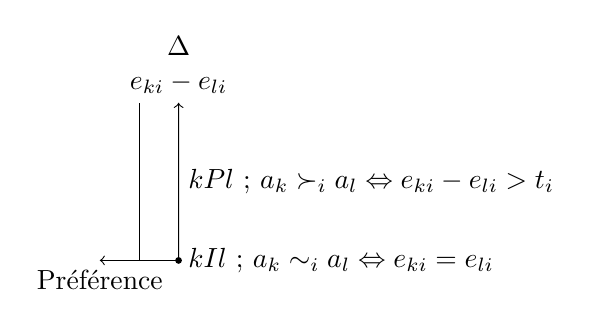
\begin{tikzpicture} %[?options?] 
%  ?tikz commands?
\draw [->] (0,0) -- (0,2);
\filldraw
(0,0) circle (1pt) --
(0,2) node[align=center, above] {$\Delta$\\$e_{ki} - e_{li}$} --
(0,1) node[align=center, right] {$kPl$ ; $a_{k} \succ_{i} a_{l} \Leftrightarrow e_{ki} - e_{li} > t_i$} --
%(0,4) circle (1pt) node[align=center, left] {t}
%(0,4) circle (1pt) node[align=center, right] {seuil entre préférence faible et préférence strict} --
%(0,3) node[align=center, right] {$kQl$ ; $ a_{k} \succsim_{i} a_{l} \Leftrightarrow q_i < e_{ki} - e_{li} \leq t_i $} --
%(0,2) circle (1pt) node[align=left, left] {q}
%(0,2) circle (1pt) node[align=left, right] {seuil entre préférence faible et indiférence}     -- 
(0,0) node[align=center, right] {$kIl$ ; $ a_{k} \sim_{i} a_{l} \Leftrightarrow e_{ki} = e_{li}$};
 %node[align=center,  above] {} --;
 \draw
 (0,0) --
 (-0.5,0)--
 (-0.5,2);
 \draw [->] (0,0) -- (-1,0);
 \filldraw 
  (-1,0) node[align=left, below] {Préférence};
 
\end{tikzpicture}
\caption{Représentation de la préférence stricte. Usage d'un critère vrai.}
\label{fig:pref_strict}
\end{figure}

Les préférences suivant un ``quasi-critère'', illustrées Fig.\ref{fig:pref_strict_distancé}, se traduisent de la façon suivante~:
\begin{equation}
\begin{cases} a_{k} \succ_{i} a_{l} \Leftrightarrow e_{ki} - e_{li} > q_i & \\
a_{k} \sim_{i} a_{l} \Leftrightarrow |e_{ki} - e_{li}| \leq q_i & 
\end{cases}
\end{equation} 
Il s'agit d'une échelle ordinale avec seuil\footnote{\blockcquote[section 3.7.1.2]{bouyssou_evaluation_2006}{Ordinal scale with a threshold}}.
La supériorité stricte de la différence des évaluations d'une alternative sur l'autre au seuil d'indifférence, lui vaut la préférence stricte. Si la différence des évaluations de deux alternatives est inférieure au seuil d'indifférence, par exemple un ordre de grandeur déterminé par un intervalle d'incertitude de l'évaluation, alors aucune des alternatives n'est préférable.

\begin{figure}
\centering
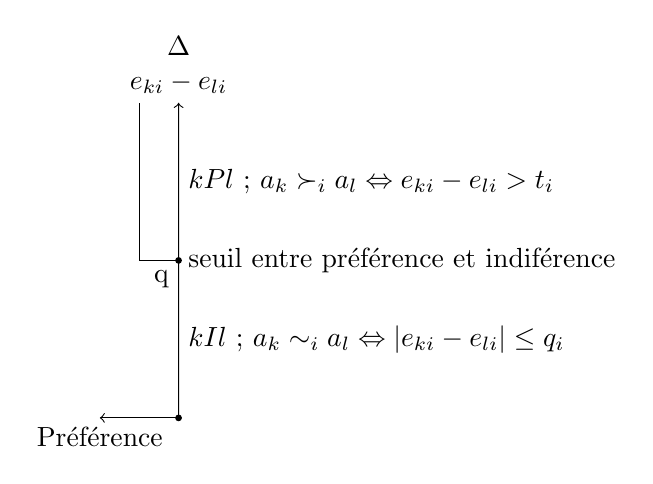
\begin{tikzpicture} %[?options?] 
%  ?tikz commands?
\draw [->] (0,0) -- (0,4);
\filldraw
(0,0) circle (1pt) --
(0,4) node[align=center, above] {$\Delta$\\$e_{ki} - e_{li}$} --
(0,3) node[align=center, right] {$kPl$ ; $a_{k} \succ_{i} a_{l} \Leftrightarrow e_{ki} - e_{li} > t_i$} --
%(0,4) circle (1pt) node[align=center, left] {t}
%(0,4) circle (1pt) node[align=center, right] {seuil entre préférence faible et préférence strict} --
%(0,3) node[align=center, right] {$kQl$ ; $ a_{k} \succsim_{i} a_{l} \Leftrightarrow q_i < e_{ki} - e_{li} \leq t_i $} --
(0,2) circle (1pt) node[align=left, below left] {q}
(0,2) circle (1pt) node[align=left, right] {seuil entre préférence et indiférence}     -- 
(0,1) node[align=center, right] {$kIl$ ; $ a_{k} \sim_{i} a_{l} \Leftrightarrow |e_{ki} - e_{li}| \leq q_i$};
 %node[align=center,  above] {} --;
  \draw
  (0,0) --
  (0,2) --
  (-0.5,2)--
  (-0.5,4);
  \draw [->] (0,0) -- (-1,0);
  \filldraw 
   (-1,0) node[align=left, below] {Préférence};
\end{tikzpicture}
\caption{Représentation de la préférence stricte avec distance. Usage de quasi-critère}
\label{fig:pref_strict_distancé}
\end{figure}

Les préférences suivant un ``pseudo-critère'', illustrées Fig.\ref{fig:weak_pref}, se traduisent de la façon suivante~\footnote{Les seuils q et t sont également exprimés en littérature par x' et x''~\cite{bouyssou_evaluation_2006}}~:
\begin{equation}
\begin{cases} a_{k} \succ_{i} a_{l} \Leftrightarrow e_{ki} - e_{li} > t_i &  \\
a_{k} \succsim_{i} a_{l} \Leftrightarrow q_i < e_{ki} - e_{li} \leq t_i & \\
a_{k} \sim_{i} a_{l} \Leftrightarrow |e_{ki} - e_{li}| \leq q_i & 
\end{cases}
\end{equation} 
%\colorbox{yellow}{probable erreur dans l'article de Rowley, relire jusqu'à validation puis mail à Hazel.}

\begin{figure}
\centering
\begin{tikzpicture} %[?options?] 
%  ?tikz commands?
\draw [->] (0,0) -- (0,6);
\filldraw
(0,0) circle (1pt) --
(0,6) node[align=center, above] {$\Delta$\\$e_{ki} - e_{li}$} --
(0,5) node[align=center, right] {$kPl$ ; $a_{k} \succ_{i} a_{l} \Leftrightarrow e_{ki} - e_{li} > t_i$} --
(0,4) circle (1pt) node[align=center, left] {t}
(0,4) circle (1pt) node[align=center, right] {seuil entre préférence faible et préférence strict} --
(0,3) node[align=center, right] {$kQl$ ; $ a_{k} \succsim_{i} a_{l} \Leftrightarrow q_i < e_{ki} - e_{li} \leq t_i $} --
(0,2) circle (1pt) node[align=left, below left] {q}
(0,2) circle (1pt) node[align=left, right] {seuil entre préférence faible et indiférence}     -- 
(0,1) node[align=center, right] {$kIl$ ; $ a_{k} \sim_{i} a_{l} \Leftrightarrow |e_{ki} - e_{li}| \leq q_i$};
 %node[align=center,  above] {} --;
 \draw
   (0,0) --
   (0,2) --
   (-0.5,2)--
   (-0.5,4)--
   (-1,4)--
   (-1,6);
   \draw [->] (0,0) -- (-1.5,0);
   \filldraw 
    (-1,0) node[align=left, below] {Préférence};
\end{tikzpicture}
\caption{Représentation de la préférence faible. Usage de pseudo-critère}
\label{fig:weak_pref}
\end{figure}
Il s'agit d'une échelle ordinale à deux seuils\footnote{\blockcquote[section 3.7.1.2]{bouyssou_evaluation_2006}{Ordinal scale with two thresholds}}.
La supériorité stricte de la différence des évaluations d'une alternative sur l'autre au seuil d'indifférence, lui vaut la préférence stricte.
La préférence faible ($\succsim$) intervient lorsque la différence des évaluations se situe entre deux seuils.
Un premier seuil peut représenter l'incertitude.
Le second peut indiquer une \emph{``distance significative''} entre les intervalles d'incertitudes.
Si la différence des évaluations de deux alternatives est inférieure au seuil d'indifférence, par exemple l'intervalle d'incertitude de l'évaluation, alors aucune des alternatives n'est jugée préférable.

Les nuances de préférences sont généralisables de façon discrète avec n seuils~\cite[3.7.1.4 Ordinal scale with k thresholds]{bouyssou_evaluation_2006}.
Les formes de préférences peuvent aussi êtres définies de façon continue (CF les dernières modalités
%de la figure~\ref{fig:pref_PROMETHEE},
dans la méthode \gls{PROMETHEE}, avec critère gaussien).

%???????????????????
%
%Autres formes de seuils, limites exclusion supérieure et inférieure
%
%? incomparabilité et ELECTRE
%
%\citetitle{roy_outranking_1991}
%\citeauthor{roy_outranking_1991}
%\cite{roy_outranking_1991}
%
%
%
%À partir des quasi- ou pseudo- critère, différentes relations de préférence peuvent être établies\blockcquote{boufateh_ben_arari_contribution_2011}{La fonction de préférence de a par rapport à b au jème critère est Fj(a,b), un nombre compris entre 0 et 1 qui croît avec l'écart gj(a) ? gj(b) en fonction de la manière dont la préférence est modélisée (figure 2.3)'']}.
%Ces relations sont également décrites par \citeauthor{deshmukh_preference_2013}.
%???????????????????

%\colorbox{red}{idem copyright à vérifier pour le cas particulier des figures, ici thèse, fr. Pas de droit US}
%\begin{figure}[h]
%\begin{center}
%%\begin{figure}[r]
%\includegraphics[width=14cm]{/home/rudy/Documents/rudy/01_These/11_production/01_COMMUNICATION/figures_extraites/Boufateh_2011_promethee_preferences.pdf}
%\caption{Formes de préférence sous PROMETHEE. Extrait de \cite{boufateh_ben_arari_contribution_2011}}
%%\end{figure}
%\label{fig:pref_PROMETHEE}
%\end{center}
%\end{figure}

%\figbox{Les lecteurs auront pu observer sur la figure\ref{fig:pref_PROMETHEE} ! \colorbox{yellow}{check rights on the graph} les parallèles de notations et descritpions de \citeauthor{bouyssou_evaluation_2006} à \citeauthor{boufateh_ben_arari_contribution_2011}.}
\subsubsection{Discussion des \textit{critères}}
Les alternatives peuvent donc être évaluées suivant des critères économiques, sociaux, de gouvernance et environnementaux, car la diversité des méthodes d'interprétation permet la prise en compte de critères (ou attributs) de natures variées.

Une grande prudence sera de mise pour la sélection ou la construction des critères.
Les critères pour être employés au sein d'une \gls{PAMC} sont de préférence~: %d'après \citeauthor{rowley_aggregating_2012} et \citeauthor{bouyssou_evaluation_2006}
``exhaustifs, en quantité minimale, monotones, cumulatifs et indépendants'', \citeauthor{rowley_aggregating_2012} citant (Bouyssou (1990)\footnote{Bouyssou, D., 1990. Building criteria: a prerequisite for MCDA. In: Bana e Costa, C.A. (Ed.), Readings in Multiple Criteria Decision Aid. Springer-Verlag, Berlin, pp. 58e80. Nous n'avons su accéder à cette référence.})\cite[p.27 (p.4 de l'article)]{rowley_aggregating_2012}.
\citeauthor{moullec_towards_2014} lorsqu'elle liste les critères indiqués par Bouyssou 1990 (semble-t-il la même référence) ne retiens que "Exhaustiveness ; Monotonicity ; Non-redundancy"~\cite{moullec_towards_2014}.

%\colorbox{yellow}{? ref bouyssou non accessible > faire un lien sur la partie de discussion des indicateurs (tous "liés et non indépendants)}
%
%
%??? Section spécifique sur les indicateurs ???
\label{sec:indépendance des indicateurs}
Plus particulièrement l'indépendance semble difficilement atteignable avec l'intégration du Life Cycle Costing et de l'\gls{ACVS}.
Rien qu'au sein du seul domaine \emph{environnemental} de l'\gls{ACV}, l'indépendance est délicate.
Peut-on sans autre précaution affirmer que l'indicateur d'épuisement des ressources d'énergie fossiles, l'indicateur de potentiel de réchauffement global et l'indicateur d'émission de particule avec son impact sur la santé humaine sont indépendants~\barre{?}~!
Sur les dimensions sociale et économique, la liaison des indicateurs est indéniable.


\exbox{
Pour reprendre la théorie de la valeur sous la formule de J.M. Jancovici, ``l'argent n'achète que des hommes''\footnote{Formule qu'il emploi dans "C'est maintenant !", co-écrit avec Alain Grandjean, 2009.}.
Considérons le cadre du travail salarié et des préférences sur les indicateurs monétaires et imaginons des alternatives parmi lesquelles il faudrait choisir.
Optons d'une part pour une \textbf{préférence décroissante de leurs coûts} respectifs (on veut acheter la moins chère).
Et d'autre part posons une \textbf{préférence croissante sur l'emploi} que les alternatives génèrent (on veut plus de travail salarié).
Cela fait apparaître par la dépendance des indicateurs une \textbf{contradiction évidente}.
Les orientations contradictoires de la préférence d'un indicateur sur l'autre sont dignes d'intérêt pour la société.
Ces deux critères sont très clairement liés par le taux horaire de rémunération applicable aux masses salariales concernées.
C'est donc le jugement de valeurs des parties prenantes qui doit faire pencher la décision vers une aire de protection (une forme de richesse ou de valeur en son sens le plus large), ou une autre.
La contradiction doit éclairer que ce qui est souhaité n'est pas la subordination (l'emploi), mais l'accès aux conditions d’existence.
Ajouter à cette première réflexion des modèles alternatifs d'obtention des condition matérielles d'existence qu'un \emph{revenu} et l'indicateur de chômage, de \emph{non-emploi}, d'\emph{absence de subordination contractualisée}, n'est plus observé avec une préférence croissante suivant la même orientation (préférence vers le moindre état de subordination).
}

Pour revenir aux caractéristiques des critères, selon \citeauthor{rowley_aggregating_2012} rappelant (\textsc{Bouyssou} 1990), il semble difficile d'obtenir \textbf{l'indépendance des critères}.
Les auteurs nous alertent sur les effets de double comptage.
Mais l'indépendance de l'ensemble des critères est-elle tout simplement nécessaire à la décision~?
Faut-il retenir la synthèse de \textsc{Moullec} ou de \textsc{Rowley} et quel éclairage pouvons nous y apporter~?
Le traitement ultérieur des critères doit être considérée pour prendre position.

\keybox{
Le fait que deux critères (corrélés ou liés causalement) évoluent de paires et dégradent un scénario considéré n'ôte pas le fait que pour ledit scénario, deux signaux négatifs \emph{sont et doivent} être perçus par les parties prenantes et le décideur.
Mais cela va plus loin.
En questionnant l'indépendance, nous nous apercevons que la redondance est question du système de valeur et non une caractéristique intrinsèque du set de critères choisi.
\textbf{Avant même leur pondération, la détermination des critères} (exhaustifs, monotones, non-redondants) \textbf{dépend donc du système de valeurs.}
}
\exbox{
Prenons deux séries d'exemples.

Si un baril de pétrole est brûlé, il réduit les ressources des générations à venir \textbf{et} engendre un forçage radiatif supplémentaire.
En suivant ces deux indicateurs (GWP, RD), fonctionnellement liés (non-indépendant), s'expriment deux conséquences négatives, significatives pour le décideur.
Bien que liées, la prise en compte de ces deux indications n'est pas un double comptage.
Les deux conséquences sont distinctes.

Considérons maintenant un indicateur tel l'énergie totale cumulée, \gls{CED}. %(CED Cumulated Energy Demand).
Employée avec un \gls{GWP} et/ou \gls{RD}, l'indication pourrait être qualifiée de redondante.
Une quantité d'énergie employée (niveau d'information "Inventaire"), n'indique en rien une conséquence (impact ou dommage).
Les trois indicateurs iront probablement de pairs.

Maintenant, si pour un système de valeur particulier, l'usage même de l'énergie est perçu comme affectant une valeur (i.e. qui génère un impact ou un dommage), alors la \gls{CED} pourrait être considérée comme non-redondante.
L'indicateur \gls{RD} se voit d'ailleurs parfois décomposé (\gls{RD} fossiles, renouvelable).
Il peut donc bien y avoir distinction de ces indicateurs corrélés sans double comptage, sous réserve de considérer les nuances attenantes.

Considérons maintenant pour seconde série, dans une même étude pour une même décision deux indicateurs~:
\begin{itemize}
\item L'impact sanitaire d'une activité (thème ``health \& safety'') au travers un indicateur social tel que proposé dans les travaux de \citeauthor{benoit-norris_identifying_2012}~\cite{benoit-norris_identifying_2012}
\item et les indicateurs de l'aire de protection ``santé humaine'' de l'\gls{ACV} tel que dans\citetitle{jolliet_impact_2003} ~\cite{jolliet_impact_2003} (par exemple)
\end{itemize}
La prise en compte simultanée des deux indicateurs engendre-t-elle un double comptage ?
Il s'agit de compartiments différents, l'ambiance de l'environnement de travail (``working environment'', indicateur sociaux ou sanitaire sur les conditions de travail) \emph{dans la techno-sphère} et l'atmosphère extérieure, représentée dans l'\gls{ACV} évaluant les échanges \emph{avec la biosphère}.
De plus il s'agit dans les deux cas de transmettre des pathologies à l'Homme.
Il y a cependant peut-être communication de l'ambiance de travail à l'environnement extérieur (aspiration pour rejet à l'atmosphère).
Ici c'est le rejet de la présence de composants de la biosphère au sein de la techno-sphère qui est problématique.
Considérer qu'il s'agit des mêmes phénomènes et que la distinction biosphère VS techno-sphère est une construction dépassée par les modèles par compartiments résout l'affaire en n'en faisant qu'un seul indicateur dont les facteurs d'impacts seront associés aux parcours et au devenir probables des substances (fate and pathways).

Toutefois si nous considérons comme situations particulières avec des facteurs tels~: \emph{l'exposition sous subordination} ; en connaissance de cause ou non ; l'exposition d'un tiers sans lien à l'activité, voir à son insu, etc. \emph{il s'agit d'indications spécifiques.}
La mesure précise par compartiment des émissions deviendra plus critique (pour éviter le double comptage ou l'absence de comptabilisation).
Bien que non-indépendants ces critères de santé considérés séparément ne sont plus \emph{redondants} entre eux.
}
%\colorbox{yellow}{? dans chap sur description et indicateurs ?}

Nous venons de le voir en exemple, le questionnement sur l'unicité, la redondance et l'indépendance nécessite une réflexion particulière.
Cette réflexion est probablement incompatible avec un processus séquentiel sans retour sur la liste de critères établis.
Ainsi, l'ordonnancement apparent des tâches avec\begin{enumerate}
\item (i) la détermination des dimensions observées et
\item (ii) la formulation des formes de préférences sur celles-ci
\end{enumerate}

reste logique mais nécessite une démarche itérative pour que les capacités cognitives humaines limitées ne réduisent pas par heuristique le nombre de dimensions observées.
Ceci nous induira lors de la reconception critique de l'ACV à réclamer~: \emph{non-pas un état fixe du système d'interprétation avant l'étude, mais sa transparence tout au long du processus.}

\subsubsection{Des méthodes d'\gls{ADMC}}
Les quasi- et pseudo- critères ainsi que les quatres relations types sont implémentés au travers des différentes versions d'outils d'\gls{ADMC}.

Citons \textsc{Promethee}
 %Preference Ranking Organization METhod For Enrichment Evaluation
 \footnote{Brans JP, Mareschal B, Vincke P. PROMETHEE: A new family of outranking methods in multicriteria analysis. JP Brans (ed), Operational Research?84, Elsevier Science Publishers BV (North-Holland); 84:408?421; 1984.}.
%\colorbox{yellow}{reprendre des références en livre bouyssou et Triantaphyllou}
Présentée par \citeauthor{deshmukh_preference_2013} dans \citetitle{deshmukh_preference_2013}, de la version I à VI il est clairement stipulé dès le résumé que~:
\blockcquote[traduction]{deshmukh_preference_2013}{
Les informations demandées par PROMETHEE sont particulièrement claires et faciles à définir pour les décideurs et les analystes.
Il s'agit de fonctions de préférence associées à chaque critère, ainsi que des poids décrivant leur importance relative.
%The information requested by PROMETHEE is particularly clear and easy to define for both decision-makers and analysts.
%It consists in a preference function associated to each criterion as well as weights describing their relative importance.
}
%\footnote{
Si \citeauthor{deshmukh_preference_2013} les qualifie de 'facile à définir', nous recommandons cependant l'usage de technique d'assistance.
Nous traiterons cela avec l'\acrshort{AHP}.
%}
%\item 

Mentionnons également \textsc{Electre}, ELimination Et Choix Traduisant la REalité\footnote{R. BENAYOUN, B. ROY, B. SUSSMANN, ELECTRE
: Une méthode pour guider le choix en présence de points de vue multiples, Note de travail n° 49 de la Direction Scientifique de la SEMA, juin 1966.},
proposé par \citeauthor{roy_classement_1968} dans \citetitle{roy_classement_1968}~\cite{roy_classement_1968}\footnote{
Développée sur une génération (68-91) \citetitle{roy_outranking_1991}~\cite{roy_outranking_1991}.}.

Ces deux familles récentes de méthodes (\textsc{Electre} et \textsc{Promethee}) nous parraissent parfaitement pertinentes pour pour les critères quantitatifs et chargés d'incertitude que nous rencontrons en \gls{ACV}.
Mais l'histoire des \gls{ADMC} n'est pas neuve et le panel de méthodes est plus varié que celles dont nous avons connaissance.
\textsc{Condorcet} (1743-1794) et son paradoxe sur les systèmes de votes font l'exemple du travail de longue date sur la thématique.
Dans le cadre de nos travaux sur la soutenabilité, \citetitle{arrow_difficulty_1950} doit être reconnue.
Dans cet article \citeauthor{arrow_difficulty_1950}
\footnote{
\blockcquote{arrow_difficulty_1950}{This paper is based on research carried on at the \textbf{RAND- Corporation}}.
Il s'agit bien des mêmes que pour la société des eaux néerlandaises.
}
énonce le Théorème d'impossibilité (ou paradoxe d'Arrow)~\cite{arrow_difficulty_1950}.
\label{Annexe:Arrow}

Le rappel de l'expression original des conditions et de l'impossibilité est fait en~\ref{Arrow},
voici leur reprise.
\begin{itemize}
\item Non-dictature~: La préférence d'un groupe d'individus n'est pas imposé par une unique personne.
\item Souveraineté~: Les préférences ne peuvent être imposées ou définie comme un ordre pré-existant.
\item Monotonie~: Il n'est pas possible de 'descendre' une alternative dans le classement par l'action d'un individu lui attribuant une importance plus 'haute'.
\item Indépendance des alternatives non-pertinentes~:
\exbox{
Pour illustrer cette condition, observons la chose suivante~:
prenons les alternatives x, y, z et w et les individus I, II et III les ordonnant avec la plus haute valeur pour la préférée.

\begin{center}
$
\begin{matrix}
      & x & y & z & w\\
I     & 4 & 3 & 2 & 1\\
II    & 4 & 3 & 2 & 1\\
III   & 2 & 1 & 4 & 3\\
Somme & 10 & 7 & 8 & 5\\
\end{matrix}
$
\end{center}

L’ordonnancement est donc x, z, y, w.

Maintenant considérons l'absence de l'alternative y.

\begin{center}
$
\begin{matrix}
      & x & z & w\\
I     & 3 & 2 & 1\\
II    & 3 & 2 & 1\\
III   & 1 & 3 & 2\\
Somme & 7 & 7 & 4\\
\end{matrix}
$
\end{center}

Il y a indétermination ou indifférence entre x et z. (ou xIz)

La condition imposée par \citeauthor{arrow_difficulty_1950} est que l'ordre x, z, w soit maintenu par l’existence antérieure de l'ordonnancement x, z, y, w.

Dans nos exercices d'\gls{ACV}, il est toutefois plus fréquent d'identifier des alternatives \textit{a posteriori} et donc d’accroître le nombre d'alternative et non de le réduire.
}
\item Universalité~: pour chaque expression de préférence identique, la solution est un unique ordre complet (pas d'indétermination).
\end{itemize}

Les suites de l’énoncé (en termes de recherche) furent de questionner chacune des conditions et sa \textit{nécessité} ainsi que les conséquences de son absence.
C'est dans la volonté d'une unique voie unanimement reconnue au sein d'un groupe qui, d'après nous, nous laisse dans l'impasse.
Nous allons traiter cette question avec une autre méthode, l'\acrshort{AHP}.

\subsubsection{Architecture des valeurs, l'\acrshort{AHP}}
\label{subsubsec:AHP}
L'\acrshort{AHP}, le processus analytique de hiérarchisation
\footnote{
Processus analytique de hiérarchisation, traduit de 'Analytic Hierarchy Process'.
Saaty, T. (1972). An eigenvalue allocation model for prioritization and planning. In Working paper, Energy Management and Policy Center: University of Pennsylvania.

Saaty, T.L., “A scaling method for priorities in hierarchical structures,” Journal of Mathematical Psychology , Vol. 15, No. 3, pp. 234-281,1977.
}
bénéficie d'un large spectre d'applications et donc du retour d'expérience attenant~\cite{vaidya_analytic_2006}
\footnote{\citeauthor{vaidya_analytic_2006}référence 150 articles d'application. Domaines d'application~: Personnel, Social, Éducation, Ingénierie, Fabrication, Industrie, Politique, Gouvernement}.
Elle a également été développé dans le cadre de décision en large groupe (LGDM large groupe decision making)~\cite{liu_method_2016}.

La méthode dans sont plus simple appareil consiste en la confrontation par paire d'éléments pour la détermination de leur importance relative.
Je présente ceci graphiquement,
inspiré par le figure aux pommes de \citeauthor{saaty_fundamentals_2004}~\cite{saaty_fundamentals_2004}, je la révise pour étendre mon propos.

Sur la base d'une échelle d'entiers allant de 1 à 9 (table~\ref{tab:saaty_echelle}), l'utilisateur oppose les composants de la paire.
\begin{table}
\centering
\caption{Échelle fondamentale\cite{saaty_decision_2004}.}
\begin{tabular}{ l l }
\hline
Valeur & Importance relative \\
\hline
1 & Égal importance  \\ 
2 & Faible \\ 
3 & Modérée \\ 
4 & Modérée plus \\ 
5 & Forte importance  \\ 
6 & Forte plus \\ 
7 & Vraiment forte ou démontrée  \\ 
8 & Vraiment plus forte \\ 
9 & Extrême importance \\ 
\hline
\end{tabular}
\label{tab:saaty_echelle}
\end{table}

\begin{figure}[htbp]
\centering
	\caption{Principe de la matrice de comparaison par paire, inspirée par \citeauthor{saaty_decision_2004}~\cite{saaty_decision_2004}}
%	\vspace{-0.2cm}
	\includegraphics[width=\linewidth]{/home/rudy/Documents/rudy/01_These/11_production/01_COMMUNICATION/figures/AHP_comparison_matrix_principle.pdf}
	\label{fig:matrix_saaty_revised}
\end{figure}
\figbox{
Les rapports d'importance dans la figure~\ref{fig:matrix_saaty_revised} se construisent de la façon suivante.

Si le réceptacle A est jugé modérément supérieur au B, le rapport C1/C2 prendra la valeur 3/1.
De façon consistante et réciproque, le rapport de C2/C1 vaudra 1/3.
etc.
}
Les priorités sont déterminées selon diverses techniques.
\citeauthor{saaty_fundamentals_2004} emploie et défend le vecteur propre principal droit (`principal right eigenvector').
Quatre méthodes sont exposées par \citeauthor{ishizaka_how_2006}\footnote{\citeauthor{barzilai_consistency_1998} propose également l'extraction de la part consistante sans révision de l'inconsistance~\cite{barzilai_consistency_1998}.} avec pour conclusion que les écarts n’apparaissent qu'entre alternatives proches et de façon croissante avec l'introduction d'inconsistance~\cite{ishizaka_how_2006}.
Ceci nous pousse à \emph{ne pas choisir une} méthode mais à les balayer ainsi qu'à explorer l'inconsistance et son origine.

La réalité ne nous permet que rarement d'être consistent.
%Reality scarcely enables us to be consistent.
		%		\includegraphics[width=0.5\linewidth]{/home/rudy/Documents/rudy/01_These/11_production/01_COMMUNICATION/figures_extraites/wikicommons/AHP/Veuve_clicquot_bottle_sizes.jpg}
%		 to 30~L for a Melchizedek or Midas of Champagne. An original standard jerrycan holds 20~L.
La problématique ne se limite pas à la critique de l'échelle numérique du classement de 1 à 9 (contenant donc beaucoup de nombres premiers pour 9 niveaux)\footnote{Il s'est avéré délicat de produire des matrices 3*3 consistantes sans (ab)user des multiples 3-6-9.}.
Ainsi, des  \href{https://en.wikipedia.org/wiki/Wine_bottle#Sizes}{bouteilles de tailles variées}, de 0.1875~L avec un piccolo à un Melchizedek ou Midas de Champagne de 30~L, comme un verre \href{http://thechive.com/2011/07/20/you-should-have-a-drink-worlds-biggest-beverages-16-photos/}{\textcolor{magenta}{pouvant contenir une personne}}, bref la distribution des entités comparées paire à paire, perturbe nos hiérarchisations.

Il y a bien entendu des développement avec préférence floue, (Fuzzy AHP)~\cite{hanine_new_2016}.
Mais ce que nous retenons des travaux de \citeauthor{saaty_decision_2004}, c'est que l’inconsistance reste utile pour développer nos systèmes de valeurs~\cite[5. From Consistency to Inconsistency]{saaty_decision_2004}.
En conséquence, plus que de réduire l'inconsistance du jugement par l'extraction d'une fraction consistante ou d'une déformation de celui-ci vers la consistance, il s'agit plus d'étendre le nombre de dimensions discutées sur la base des inconsistances remontées
\footnote{
\blockcquote[traduction]{saaty_decision_2004}{
Ainsi, nous vivons avec la contradiction que nous devons être cohérents pour capturer des connaissances valides sur le monde, mais en même temps, être prêt à changer nos états d'esprits et être inconsistant si de nouvelles informations exigent que nous pensions différemment d'auparavant.
%Thus we live with the contradiction that we must be consistent to capture valid knowledge about the world but at the same time be ready to change our minds and be inconsistent if new information requires that we think differently than we thought before.
}
}.
En somme, si nous présentons et utilisons cette méthode, ce n'est pas pour produire la sélection des alternatives, mais pour conduire une réflexion axiologique.
% Axiological thinking is not simpler.
%		
%		Not limited to AHP.
%		What matters: the 'consistence' between decision-maker's values and the used technique.

\subsection{D'autres types de méthodes~?}

\citeauthor{rowley_aggregating_2012} indique également des méthodes n'impliquant pas le décideur.
\blockcquote[traduction]{rowley_aggregating_2012}{
D'autres méthodes ont aussi été proposées qui n'impliquent pas directement le décideur, mais au lieu de cela font l'extraction un schéma de pondération inhérent aux données elles-même.
Ces méthodes 'guidées par les données' comprennent une méthode basée sur l'enveloppement des données, une méthode d'évaluation croisée (Doyle, 1995), la méthode d'entropie (pomerol et Barba-Romero, 2000) et la méthode intégrale floue (Rowley et al., Sd) .}
%Other methods have also been proposed which do not directly involve the decision maker but instead extract a weighting scheme inherent to the dataset itself. These ‘data-driven’ methods include a data envelopment analysis-based alternative cross-evaluation method (Doyle, 1995), the entropy method (Pomerol and Barba-Romero, 2000) and the fuzzy integral method (Rowley et al., n.d).}

\citeauthor*{doyle_multiattribute_1995} dans \citetitle{doyle_multiattribute_1995} propose la chose suivante.
\blockcquote[traduction]{doyle_multiattribute_1995}{
La première partie de la méthode, qui est l'application direct d'enveloppement de données, peut être pensée comme un processus idéalisé d'auto-évaluation dans laquelle chacune des alternatives pondère ses attributs afin de maximiser sa propre désirabilité par rapport aux autres alternatives.
Ces poids sont considérées comme définissant les préférences d'un fragment du marché.
La deuxième étape consiste à utiliser les poids optimaux de chaque alternative pour reconstruire l'ensemble du marché et donc de déduire la préférence d'un décideur moyen qui aurait besoin de choisir parmi ces alternatives.
}
%
%The first part of the method, wich is straightforward Data Envelopment Analysis (DEA), can be fought of as an idealized process of self-evaluation in wich each alternative weights the attributes in order to maximize its own desirability relative to the other alternatives.
%These weights are taken as defining the preferences of a fragment of the market.
%The second step is to use each alternative's optimal weights to reconstruct the entire market and thus to infer the preference of an average decision maker (DM) who needs to choose from among these alternatives.}

%Pomerol, J.-C., Barba-Romero, S., 2000. Multicriterion Decision in Management:
%Principles and Practice. Kluwer Academic Publishers, London.

%xxxxxxxxxxxxxxxxxxxxxxxxxxxxxxx

Nous marquons ici notre désaccord profond avec ces auteurs sur le propos suivant.
\blockcquote[traduction]{rowley_aggregating_2012}{
Bien que cela puisse \underline{sembler} contradictoire au but des \glspl{ADMC}, qui est d'\emph{intégrer les valeurs de décideurs}, de telles méthodes peuvent être \emph{la seule option viable si les autres méthodes sont inappropriées ou peu pratique}.
% Although this may seem to contradict one aim of MCDA, which is to incorporate decision-maker values, such methods may be the only viable option if other methods are unsuitable or impractical.
}
La praticité, (l’opérationnalité) est jugée ici supérieure à la présence effective du jugement de valeur du décideur.
Or il n'est pas question de sembler contradictoire, mais de l'être totalement.
Si le décideur sélectionné n'est pas capable de formuler ses valeurs, qu'un autre qui le sache le fasse ou que la décision soit reportée dans l'attente que la formulation puisse être faite par le décideur s'il est jugé que celui-ci est légitime.
Proposer une méthode de \emph{décision} sous des allures scientifiques, de calculs savants et complexes, qui prétende s'abstenir de jugements de valeurs \textsc{n'aide pas la prise de décision par le décideur}.
\emph{C'est la précipiter et la confisquer !}
\subsection{Des combinaisons}
Certaines techniques d'ADMC sont employées simultanément de façon à traiter une partie du processus de décision.
Ainsi, les méthodes de surclassement nécessitent comme indiqué précédemment des formes de préférences et des poids pour chaque attribut.
Une autre méthodes d'analyse multi-critère peut être employée pour déterminer la pondération des critères~\cite{myllyviita_impact_2014, kaya_integrated_2011, geldermann_fuzzy_2000}.
Pour reprendre une des conclusions de \citeauthor{herva_review_2013}, nous pouvons exploiter l'\gls{AHP} pour établir la pondération utiliser lors de la procédure de surclassement\footnote{
\blockcquote[traduction]{herva_review_2013}{
L'AHP et l'ANP étaient également très populaires, en particulier lors de la structuration d'un problème et ont souvent été utilisés comme une étape préliminaire à l'application des méthodes de surclassement et pour la détermination des poids.
%AHP and ANP were also very popular, especially when structuring a problem, and were frequently employed as a preliminary step to the application of outranking methods and for the determination of weights.
}
}.
Les travaux de \citeauthor{ziout_holistic_2014} font l'exemple de l'application de l'AHP pour la détermination de l'importance relative de critères.
\blockcquote[traduction]{ziout_holistic_2014}{
L'AHP, comme la plupart des méthodes, utilise la pondération des critères pour refléter les préférences de décision des décideurs.
L'utilisation et la sélection des poids des critères est crucial pour une bonne utilisation de la méthode (Kiritsis et al., 2003), la méthode AHP assure la bonne utilisation des poids des critères grâce à son indice de consistance (consistency index).
%AHP, as most methods, uses criteria weights to reflect decision makers preferences.
%The use and selection of criteria weights is crucial for proper use of the method (Kiritsis et al., 2003), AHP method insures the proper use of criteria weights through its consistency index.
}
Il s'agit donc ici d'une pondération par panel. % (les preneurs de décision : decision maker).
Le groupe est assisté dans sa pondération par la méthode AHP.
Dans cet article l'objectif est de choisir une option de revalorisation en fin de vie de produits (EOL end of life).
Le modèle \textsc{pestel} est exploité pour sélectionner la voie de revalorisation suivant les critères~: \textbf{P}olitiques, \textbf{É}conomiques, \textbf{S}ociaux, \textbf{T}echnologiques, \textbf{E}nvironnementaux et \textbf{L}égaux.
Toujours dans cet article la même méthode est employée pour définir le classement des scénarios de revalorisation~\cite{ziout_holistic_2014}.
\blockcquote{ziout_holistic_2014}{
L'AHP est utilisée pour classer ces options selon les multiples critères qui sont développés en section 3.3.
%AHP is used to rank these options according to multi-criteria which are developed in Section 3.3.
}
Deux méthodes d'agrégation complète successive sont donc employées.

Si comme d'autres nous employons l'\gls{AHP}, nous gardons à l'esprit les critiques qui lui sont faîtes.
\blockcquote{bouyssou_evaluation_2006}{
La technique utilisée dans AHP (Saaty, 1980), pour définir la valeur des poids est très sophistiquée (voir section 4.5.1).
Elle évite également demander au client pour les valeurs numériques, mais elle échoue pour la même raison que les méthodes précédentes.
Elle demande au client de comparer l'importance des critères. Mais le concept d'importance, même dans sa forme relative (plus important que), est si mal défini que les réponses données par le client et utilisés avec une procédure d'agrégation particulier peuvent ne pas refléter de façon fiable son système de valeurs.
Voir Belton and Gear (1983) et Dyer (1990).
%The technique used in AHP (Saaty, 1980), to set the value of the weights is very sophisticated (see section 4.5.1).
%It also avoids asking the client for numerical values, but it fails for the same reason as the previous methods.
%It asks the client to compare the importance of the criteria. But the concept of importance, even in its relative form (more important than), is so ill-defined that the answers given by the client and used with a particular aggregation procedure cannot reliably reflect his value system.
%See Belton and Gear (1983) and Dyer (1990).
}
Il semble donc nécessaire d'établir une plus ample co-élaboration des méthodes avec les psychologues.

\subsection{Interrogation perspective de travail}

%??OÙOÙOÙOÙOÙOÙOÙOÙOÙOÙOÙOÙOÙOÙOÙOÙOÙOÙOÙOÙ??

La lecture d'ouvrage de référence tel que \citetitle{bouyssou_evaluation_2006} notamment sur la préférence et sa traduction mathématique~ \cite[Chapitre 3]{bouyssou_evaluation_2006} doit nous interroger sur la possibilité (ou non) d'une réelle distinction entre observation et jugement, entre mesure et évaluation au sens de l'isolation de l'application du jugement de valeur.
Un outil intermédiaire avant même la question du jugement sera peut-être l'interrogation de la significativité des assertions.
\blockcquote[3.4. evaluation and meanigfulness]{bouyssou_evaluation_2006}{
En théorie classique de la mesure, une assertion est déclarée être significative si sa valeur vraie est inchangée lorsque les transformations admissibles sont appliquées aux échelles employées dans l'assertion.
%In classical measurement theory, an assertion is declared to be meaningful if its truth value is unchanged when admissible transformations are applied to the scales used in the assertion. 
}
Une évolution possible des travaux serait de caractériser systématiquement le type de transformation opérée et leur significativité.


%????????????????????????????????????????????????

Lors de l'étude des méthodes nous avons pu observer deux courants portant des similitudes sur des approches de détermination des valeurs.
En effet, la description de certaines méthodes mentionne que hors des alternatives, il est difficile de définir les préférences sur les indicateurs.
C'est la question des 'préférences exprimées' et 'préférences révélées', en trame de fond de la monétarisation.
La réflexion axiologique pour l'élicitation et l'articulation des valeurs nécessitera certainement de nombreuses boucles en un processus long et continu.


%\colorbox{yellow}{à relocaliser !}
La non-compensation nécessaire au concept de soutenabilité forte semble exclure des méthodes disponibles celles d'agrégation complète pour la sélection du choix final.
Toutefois, ne peut-on pas élargir nos possibilités ?
Posons des scores uniques (résultat agrégés) de différentes alternatives égaux (mathématiquement) comme incomparable (sémantiquement).
Y'aurait-il une décision finale différente, sur la base d'une même caractérisation et de poids identiques, interprétée suivant des agrégations partielles et complètes ?
\begin{figure}[htbp]
\centering
	\caption{Préférences et perspectives}
%	\vspace{-0.2cm}
	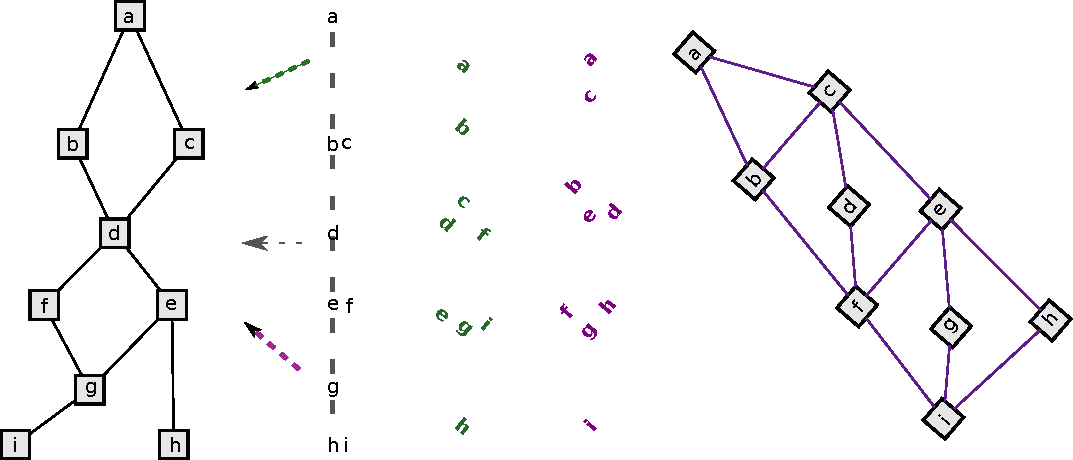
\includegraphics[width=0.7\linewidth]{/home/rudy/Documents/rudy/01_These/11_production/01_COMMUNICATION/figures/preferences_reseau_perspectives.pdf}
	\label{fig:preferences_perspectives}
\end{figure}
\figbox{
Lecture, de la représentation Fig.\ref{fig:preferences_perspectives}.
Dans quelle mesure des techniques différentes (agrégation complète, liste ordonnée ou réseau de préférences) et des perspectives différentes (figurativement avec l'inclinaison du réseau) ) modifient-elles les relations perçues entre entités et les décisions consécutives ?
Dans quelle mesure la perspective choisie sur les relations entre entités affecte-t-elle la décision\footnote{Il s'agit évidement d'une représentation figurative, les n dimensions alimentant la préférence ne sont pas réductibles à un plan de deux dimensions.} ?
Quelle est la réduction d'information minimale possible sans dépasser les seuils cognitifs et psychologiques ni déformé de façon inconsistante le jugement du décideur?
}


%\colorbox{yellow}{vers chap 4-5}

%\colorbox{yellow}{Reprendre exemple minimal avec le MMC1 de Rowley énergie coût}

%Il faut différencier les agrégations complètes pour le déterminer.
%\begin{itemize}
%\item Somme pondérée des indicateurs normalisés
%\begin{itemize}
%\item avec normalisation interne
%\item avec normalisation externe
%\end{itemize}
%\end{itemize}
%
%Cette analyse permettrait d'intégrer dans le corpus d'études soutenant la thèse d'une soutenabilité forte, des travaux sur des ''index`` de soutenabilité.
%Où comment concentrer l'information sur un indicateur unique ?
%Cela bien-sur est fait avec un grand nombre de dimensions.
%
%=> somme pondérée face à promethee face à AHP
%pressage de thèses :
%
%Moullec ? Génération de solution

Nous avons vu que l'intégration du jugement du décideur est un élément clef.
Pour présenter la question de la pluralité du corps décisionnaire, nous nous penchons sur les travaux d'\citeauthor{adla_aide_2010}.
Sans développer l'ensemble du contenu de \citetitle{adla_aide_2010}, nous observerons que la réussite d'un groupe vaste réside dans la maîtrise des communications synchrone, asynchrone, localisée et distribuée\footnote{Figure 3.3 : Quatre combinaisons des systèmes d’aide à la décision de groupe [Grudin 94], dans le Temps et l'espace~\cite{adla_aide_2010}}.

La prise en compte des parties prenantes visant la soutenabilité à l'échelle globale, tout en leur garantissant la protection de l'anonymat, \emph{est} la problématique du vote à distance (électronique).
Transparence, confidentialité, anonymat, unicité, sincérité, nous pourrions mettre tous ceci dans le cadre de l'expression du système de valeur pour la décision.
Et nous n'aurions aucun mal à reconnaître des travaux comme \citetitle{enguehard_vote_2007} de \citeauthor{enguehard_vote_2007}~\cite{enguehard_vote_2007} dans notre champ disciplinaire (ou interdisciplinaire).

La problématique de l'expression non biaisée dans les groupes distribués reste selon nous la question de `l'anonymisation-vérifiabilité' qui n'a pu être résolue jusqu'ici~\cite{pellegrini_chaines_2014}.
Il semble donc que notre espèce ne puisse accéder à ce stade de rationalité qu'en modifiant son comportement face aux expressions et au respect des opinions de chacun.e.s, pour accéder à la déclaration nominative.
Il serait naïf d'écrire cela ici sans ajouter qu'une telle occurrence est peu probable sans une horizontalisation des pouvoirs permettant de ne plus craindre d'action contre ces expressions d'opinions.
Par exemple, l'universalisation du salaire, libère de la contrainte à l'accès aux conditions matérielles d'existence.
Le tirage au sort aux fonctions de gouvernance (du local jusqu'au supra-national, tous pouvoirs confondus), libère des pressions des luttes partisanes et électives.
La co-propriété d'usage des moyens de production, libère de la subordination quant aux finalités et moyens choisis pour les obtenir.
Ne resterait donc que la coercition physique directe, difficilement extensible à de large ensemble (sous réserve des mécanismes cités précédemment).
Ces artefacts ne sont pas encore universellement appliqué ni reconnu.
Nous n'y sommes donc pas encore.


\subsection{Conclusion sur l'ADMC}
\label{concl:mcdm}

Nous avons vu au travers de cette présentation la diversité des méthodes disponibles, leurs caractéristiques et les fondements de l'\gls{ADMC}.
Nous avons ensuite traité la question des indicateurs (construction des critères) ainsi que leur formes d'agrégation, complète et partielle.
Nous en sommes venu au fait que la confrontation des deux approches doit distinguer les concepts faible et fort de la soutenabilité.
Mais en définitive, l'action de décision réside dans la mise en œuvre d'une unique alternative.
Même s'il peut s'agir de la combinaison d'alternatives, la combinaison elle-même reste une alternative unique.

La confrontation de l'école américaine et de l'école européenne (AHP, ELECTRE) est décrite par \citeauthor{lootsma_french_1990}~\cite{lootsma_french_1990}.
Elle relève par négatif les incohérences relatives aux approches de "l'évaluation objective".
C'est une indication sur l'acceptabilité de la subjectivité que nous retiendrons donc ici en conclusion.
\blockcquote[traduction]{lootsma_french_1990}{
La RAND Corporation, par exemple, une grande société de conseil américaine commanda le projet PAWN (pion) (analyse des politiques de gestion de l'eau pour les Pays-Bas, CF rapports de PAWN, 1981-1983) par l'autorité de gestion de l'eau néerlandaise `Rijkswaterstaat'
[.Elle (RAND)] a conçu un grand nombre de stratégies alternatives pour le contrôle des eaux de surface.
\emph{Ils ont rejeté l'analyse multi-critère pour la sélection finale d'une stratégie particulière, au motif que les décideurs devraient s'accorder explicitement sur les poids des critères et sur les scores des impacts.}
%The RAND Corporation, for instance, a large American consulting company commissioned with the PAWN project (Policy Analysis of Water Management for the Netherlands, see the PAWN reports, 1981-1983) by the Dutch water management authority Rijkswaterstaat, designed a large number of alternative stratégies for surface-water control.
%\emph{They rejected multi-criteria analysis for the final sélection of a particular strategy, on the ground that the decision makers would have to agree explicitly on the criterion weights and on the impact scores.
}
\keybox{
Ce qui fait obstacle à plus de rationalité dans les décisions humaines serait donc semble-t-il qu'il faille pour le décideur, être en accord avec son propre système de valeur et (pouvoir) l'assumer pleinement.
}
Toutefois, se maintenir dans l'irrationalité volontairement peut être d'autant plus préjudiciable que la solution sélectionnée peut être plus 'loin' (avec le système de valeur implicite), d'une solution plus rationnellement choisie avec le système de valeur explicite controversé mais transparent, comme d'un système plus consensuel ou d'un compromis explicité.

\keybox{
C'est en somme, au delà de l'acceptabilité de la complexité, une question de la légitimité du système de valeurs du décideur qu'il convient de résoudre pour que les \gls{ADMC}, de façon générale, et donc l'\gls{ACV} de façon particulière, soient acceptées.
} %section %%Intégrer la selection fuzzy mcdm mcda date d'ajout du 21/06/2016 avant 10h
%
\section{Conclusion sur les outils}
Qu'il s'agisse de la structuration de données ou de l'assistance à la prise de décision, la discipline de l'\gls{ACV} semble en retrait de ses sœurs aînées et voisines.
Les fondements théoriques sur la décision et la conception soulignent la criante inexistence du meilleur pour ne garder que la préférence.
Loin d'accepter dans sa majorité le rejet de \textit{l’intrinsèquement bon}, dans notre disciplines se trouvent des postures se révélant des archétypes~: du Traditionaliste dans l'appel à la simplicité, du Rationaliste constructiviste radical dans la défense de la meilleure alternative, et du Rationaliste attentiste se réclamant d'une soit disante \gls{ACV} objective de comptabilité.
Ces postures sont certainement des causes du piètre état d'élaboration des outils d'\gls{ACV} tel que vu dans ce chapitre au~\ref{sec:Outils de modélisation en ACV}.

L'\gls{ADMC} antérieure à l'\gls{ACV} a déjà entamé la liaison mais l'intégration semble lente et la communauté encore réticente 'au dépassement de la somme pondérée'.
La question du web sémantique, liées à celle de l'\emph{accessibilité des données}, cristallisant plus l'attention du praticien, dépassera peut-être la première de par le côté controversé du traitement de la subjectivité (négativement connoté) face au caractère sacré des \emph{données} dont nous sommes massivement friands et \emph{auxquelles certains d'entre nous abandonneraient même leur jugement}.

La conception fonctionnelle, semble avoir une implantation dans le tissu industriel des plus lente (au regard de sa lointaine naissance).
Sans doute est-elle aux prises avec les mêmes connotations que précédemment, puisque l'activité d'évaluation est en son sein.
Cela l'a d'ailleurs fort retardée, lorsque qualifiée d'art elle en fut (du moins un temps) dévaluée.
Elle n'en reste pas moins un outil essentiel à l'\gls{ACV} et un complément bien \textit{utile} à la décision multi-critère.

Le mouvement est lent mais les signaux sont forts concernant l'intégration de tout cela à l'\gls{ACV}.
Des cycles de re-conception méthodologique, structurés, disciplinairement soutenus et organisés sur les principes de l'open-source semblent à la fois prometteurs et en bonne voie.